\documentclass[11pt]{elegantbook}
\definecolor{structurecolor}{RGB}{40,58,129}
\linespread{1.6}
\setlength{\footskip}{20pt}
\setlength{\parindent}{0pt}
\newcommand{\argmax}{\operatornamewithlimits{argmax}}
\newcommand{\argmin}{\operatornamewithlimits{argmin}}
\elegantnewtheorem{proof}{Proof}{}{Proof}
\elegantnewtheorem{claim}{Claim}{prostyle}{Claim}
\DeclareMathOperator{\col}{col}
\title{\textbf{Unsupervised Learning}}
\author{Wenxiao Yang}
\institute{Department of Mathematics, University of Illinois at Urbana-Champaign}
\date{}
\setcounter{tocdepth}{2}
\cover{cover.jpg}
\extrainfo{All models are wrong, but some are useful.}

% modify the color in the middle of titlepage
\definecolor{customcolor}{RGB}{32,178,170}
\colorlet{coverlinecolor}{customcolor}
\usepackage{cprotect}

\addbibresource[location=local]{reference.bib} % bib

\begin{document}

\maketitle
\frontmatter
\tableofcontents
\mainmatter

\chapter{Clustering}
General Goal of \textbf{Clustering Algorithm}:
\begin{enumerate}[$\circ$]
    \item the "similarity" of the objects in the same cluster is \underline{maximized} while
    \item the "similarity" of objects in different clusters is \underline{minimized}.
\end{enumerate}

\begin{definition}
    For a given set of objects $V = \{x_1, x_2, ... , x_m\}$, we call a \textbf{cluster $\mathbf{S_k}$} a subset of these objects, and we call a \textbf{clustering} the set of all $K$ clusters $\mathbf{\{S_1 ,S_2 , ... , S_k\}}$.
\end{definition}
\begin{example}
    Clustering of $\{x_1,x_2,x_3,x_4\}$: (1). $\{\{x_1,x_3\},\{x_2,x_4\}\}$; (2). $\{\{x_1,x_3\},\{x_1,x_2,x_4\}\}$; (3). $\{\{x_3\},\{x_2,x_4\}\}$.
\end{example}

\section{K-Means}
\subsection{K-Means Clustering Optimization Problem}
\begin{enumerate}
    \item \textbf{Input:}
    \subitem Desired number of clusters (ex: $K=3$)
    \subitem Dataset of $m$ objects $X=\{\vec{x}_1,\vec{x}_2,...,\vec{x}_m\}$, where each object $\vec{x}_i=(x_{i1},x_{i2},...\vec{x}_{in})$ has $n$ numerical attributes. (We can also think of $X$ as being an $m\times n$ matrix $X_{m\times n}$.)
    \item \textbf{Goal of K-Means:}
    \subitem Out of all possible clusterings of $\{S_1 ,S_2 , ... , S_K\}$ with $K$ clusters that can be made from the $m$ objects in $X$, find the optimal clustering $\{S_1^*,S_2^*,...,S_K^*\}$ that \underline{minimizes} the sum of the "distance" of each object and the centroid (the mean of the cluster that object is assigned to).
    \subitem Technically, we can write this as an optimization problem
    \begin{equation}
        \begin{aligned}
            \{S_1^*,S_2^*,...,S_K^*\}=\argmin_{S_1,S_2,...,S_K}\sum_{k=1}^K\sum_{x\in S_k}\|x-\mu_k\|^2\\
            \textnormal{Optimal Inertia}=\min_{S_1,S_2,...,S_K}\sum_{k=1}^K\sum_{x\in S_k}\|x-\mu_k\|^2\\
        \end{aligned}
        \nonumber
    \end{equation}
    Inertia measures how well a dataset was clustered by $K$-Means. It is calculated by measuring the distance between each data point and its centroid, squaring this distance, and summing these squares across one cluster. A good model is one with low inertia \underline{and} a low number of clusters ($K$).
\end{enumerate}
Find the clustering $\{S_1^*,S_2^*,...,S_K^*\}$ that provides a \underline{global minimum} is \textbf{NP-hard}.

We use a \underline{heuristic} algorithm to find a \underline{local minimum} is good enough.

\subsection{Lloyd's Algorithm}
\begin{enumerate}
    \item \textbf{Input:}
    \subitem Desired number of clusters (ex: $K=3$)
    \subitem Dataset of $m$ objects $X=\{\vec{x}_1,\vec{x}_2,...,\vec{x}_m\}$, where each object $\vec{x}_i=(x_{i1},x_{i2},...,x_{in})$ has $n$ numerical attributes. (We can also think of $X$ as being an $m\times n$ matrix $X_{m\times n}$.)
    \item \textbf{Algorithm:}
    \begin{enumerate}[$\bullet$]
        \item \textbf{\underline{Step 1:} Centroid Initialization Step}\\
        Randomly select $K$ centroids $\{\vec{\mu}_1,\vec{\mu}_2,...,\vec{\mu}_K\}$, where $\vec{\mu}_k=(\mu_{k1},\mu_{k2},...,\mu_{kn})$
        \item \textbf{\underline{Step 2:} Cluster Assignment Step}\\
        Assign each object $x_i$ in the dataset to it's \underline{closest} centroid (specifically the \textit{smallest squared euclidean distance})
        \item \textbf{\underline{Step 3:} Centroid Update Step}\\
        Find the \underline{mean} of each cluster created in step 2. These means are now the new \underline{centroids}.
        \item \textbf{\underline{Step 4:} Stopping Criterion}\\
        If the old centroids and the new centroids are the \underline{same}, stop the algorithm. Otherwise, go back to step 2.
    \end{enumerate}
    \item \textbf{Output:} Clustering with $K$ clusters $\{V_1,V_2,...,V_K\}$.
\end{enumerate}
Lloyd's algorithm is known as a \textbf{non-deterministic} algorithm because,
even with the same input, it can exhibit different behaviors on different runs.

\subsection{Benefits and Drawbacks}
\subsubsection*{Benefits}
\begin{enumerate}[$\bullet$]
    \item Fast algorithm.
    \item Computationally efficient.
    \item It scales well as the number of objects or attributes grows really large. (However, k-means is not great for "big data".)
    \item One of the easiest to understand.
\end{enumerate}
\subsubsection*{Drawbacks}
\begin{enumerate}[$\bullet$]
    \item Only works well with some types of data.\\
    The K-means algorithm works best for data when "the underlying clustering" of the data has the following properties:
    \begin{enumerate}[(1).]
        \item Each cluster has roughly the same number of objects;
        \item The clusters are spherical;
        \item The clusters have the same sparsity;
        \item There is good separation between the clusters;
        \item You know the right number of clusters to ask for;
        \item Attributes are numerical (non-categorical);
        \item Data does not have a lot of noise or outliers.
    \end{enumerate}
    (\textbf{Caveat:} Just because some of these assumptions are not met does not mean necessarily the algorithm will perform worse.)
    \item Need to know the "right" number of clusters to ask for in advance.
    (We use k-means elbow plot method)
    \item It is a non-deterministic algorithm.
\end{enumerate}

\subsection{Elbow Method}
\subsubsection*{Elbow Plot}
\begin{enumerate}
    \item For $k=1$ to $K$:
    \subitem[a] Cluster the data several times into $k$ clusters.
    \subitem[b] Calculate the average inertia of these resulting clusterings.
    \item Plot "k vs. average inertia".
\end{enumerate}
\begin{center}\begin{figure}[htbp]
    \centering
    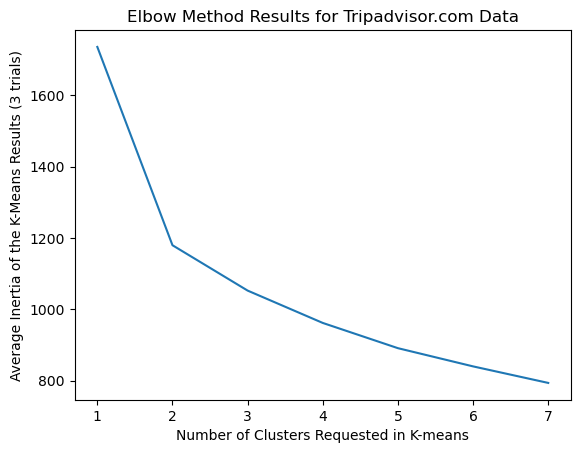
\includegraphics[scale=0.5]{elbow plot.png}
    \caption{Elbow Plot Example}
    \label{}
\end{figure}\end{center}
\subsubsection*{Interpretation of Elbow Plot}
\begin{enumerate}
    \item If there is not a dramatic elbow, then this suggests that either:
    \subitem 1. The dataset is \underline{not clusterable} or
    \subitem 2. K-means is not a suitable algorithm for detecting the underlying clusters.
    \item If there is a dramatic elbow, then this suggests that:
    \subitem 1. There is a clustering structure and
    \subitem 2. The k-means clustering algorithm is suggesting that there are about $K$ clusters where the plot levels off.
\end{enumerate}
In the example of the figure\\
1. We see a somewhat dramatic elbow in the plot. This suggests that there is some clustering structure in the dataset and that k-means is capable of identifying some clustering structure.

2. We see that that plot levels off dramatically at k=2 clusters. So this suggests that asking the k-means algorithm to return k=2 clusters will be the most insightful.

\section{Types of Clusters Definitions}
As we know the K-means algorithm can only work well with data that fulfills specific properties, we define some common \textbf{types of clusters} that could be considered in a numerical dataset to help introduce our new algorithms.

\begin{definition}[Well-Separated Cluster]
    A \textbf{well-separated cluster} defines a cluster only when the data contains natural clusters that are \underline{far apart from each other}. (This definition is vague in how far apart do clusters have to be.)
\end{definition}
Why K-means may not work well?: Well-Separated Cluster can be non-spherical.
\begin{definition}[Density-Based Cluster]
    A \textbf{density-based cluster} defines a cluster as a \underline{dense} region of objects that is surrounded by a region of \underline{lower} density. (This definition is vague in how dense it needs to be considered a cluster.)
\end{definition}
Why K-means may not work well?: Density-Based Cluster can have noise.

\begin{definition}[Graph-Based Cluster]
    \textbf{Graph-based cluster} is a group of objects that are \underline{connected} to one another, but have no \underline{connection} to objects outside the group. (This definition is vague in how do we decide objects are connected.)
\end{definition}
Why K-means may not work well?: Graph-based cluster can be non-spherical and not well separated.

\begin{definition}[Contiguity-Based Cluster (a type of graph-based
    cluster definition)]
    In \textbf{contiguity-based cluster} (a type of graph-based
    cluster definition),  two objects are \underline{connected} only if they are within a \underline{specified distance} of one another.
\end{definition}
\underline{Types of contiguity-based clustering algorithms:} spectral clustering.
\begin{center}\begin{figure}[htbp]
    \centering
    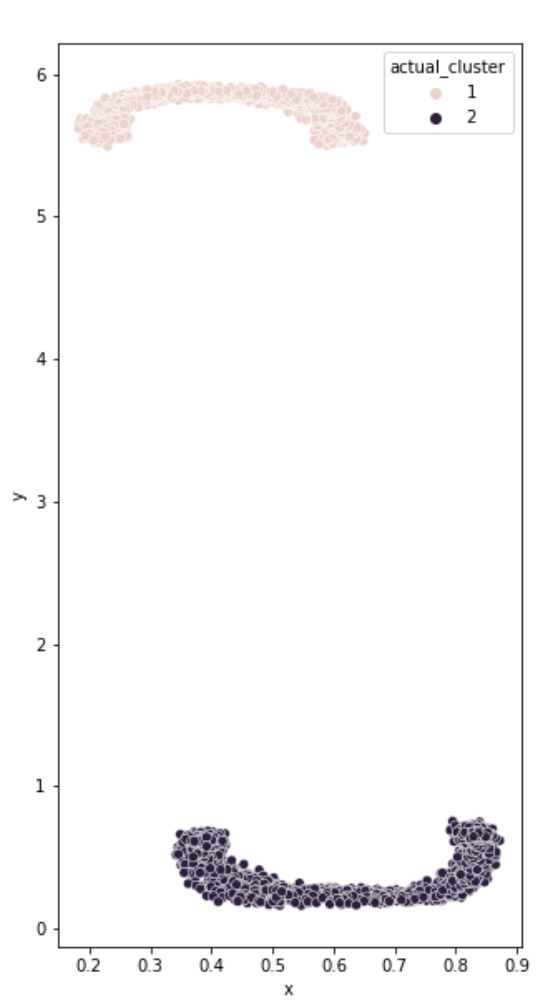
\includegraphics[scale=0.25]{well-separated.png}
    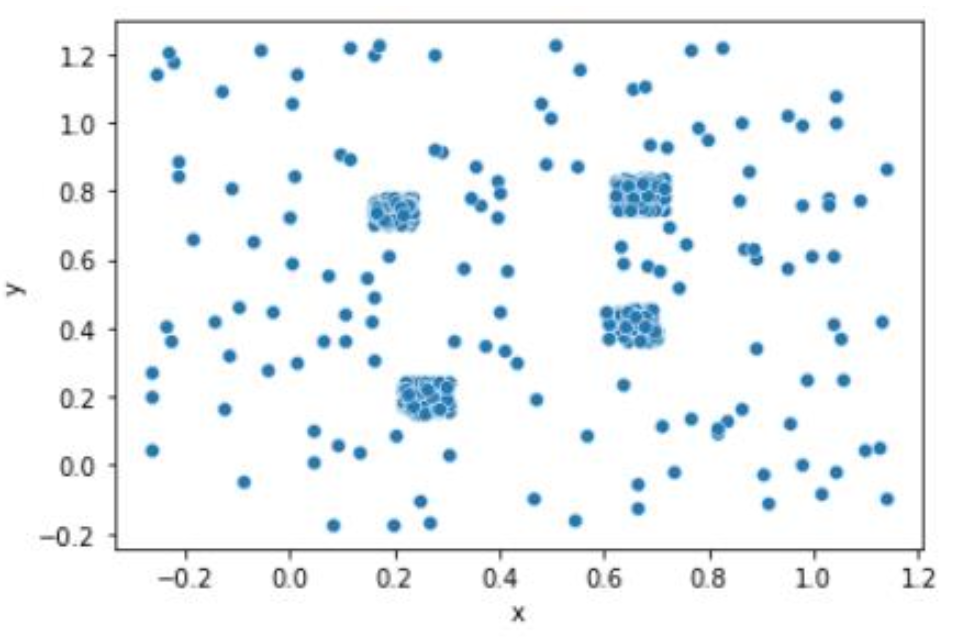
\includegraphics[scale=0.25]{density-based.png}
    \caption{(1). Well-Separated Cluster; (2). Density-Based Cluster}
    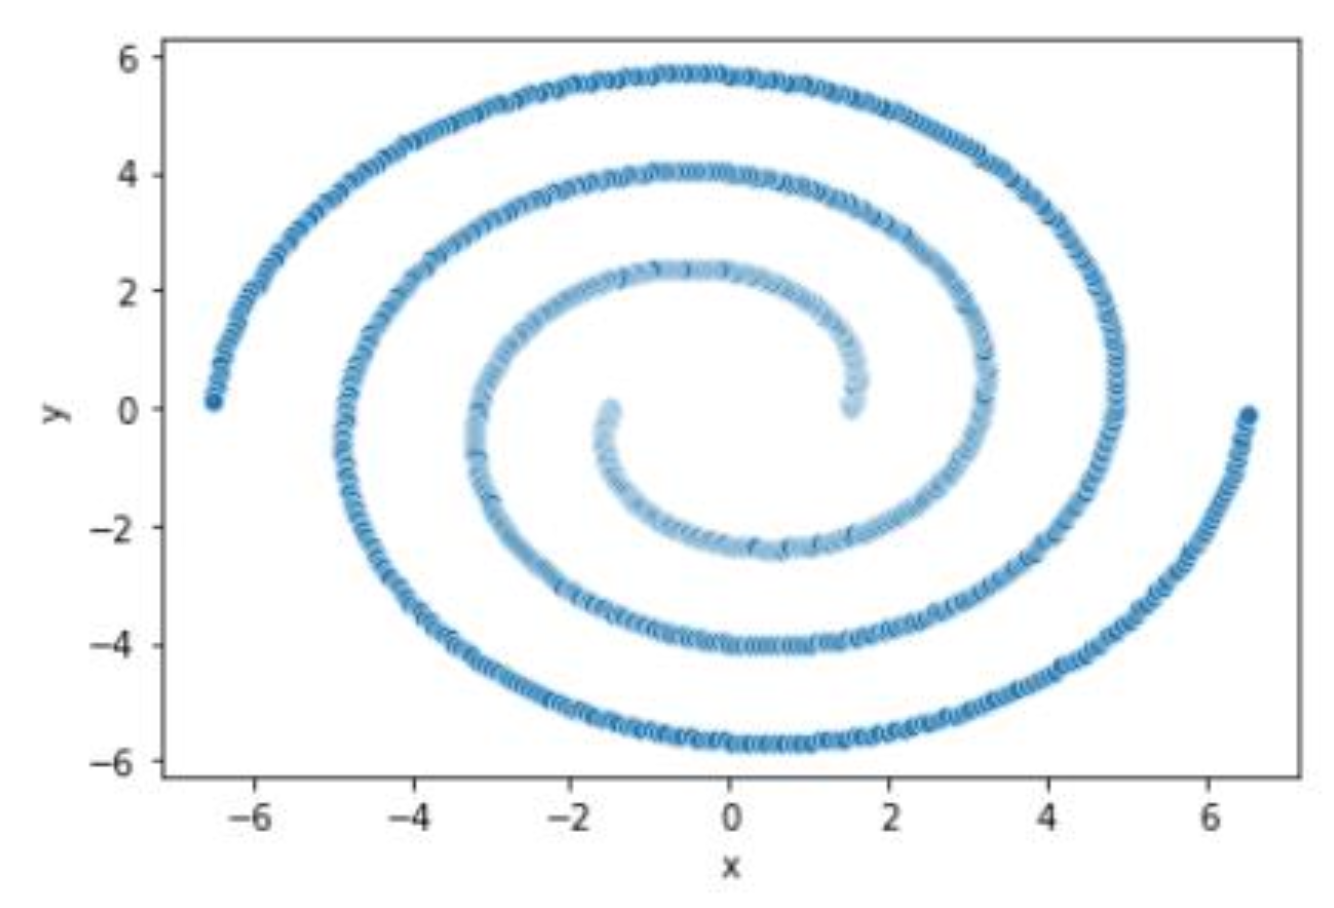
\includegraphics[scale=0.2]{Contiguity-based.png}
    \caption{Contiguity-Based Cluster}
\end{figure}\end{center}

\begin{definition}[Prototype-Based Cluster]
    A \textbf{prototype-based cluster} defines a cluster as a set of objects in which each object is closer (or more similar) to the \underline{prototype} (e.g. mean, median) that defines the cluster than to the \underline{prototype} of any other cluster.
\end{definition}
Why K-means may not work well?: Prototype-Based Cluster may be not well-separated and have outliers.
\begin{center}\begin{figure}[htbp]
    \centering
    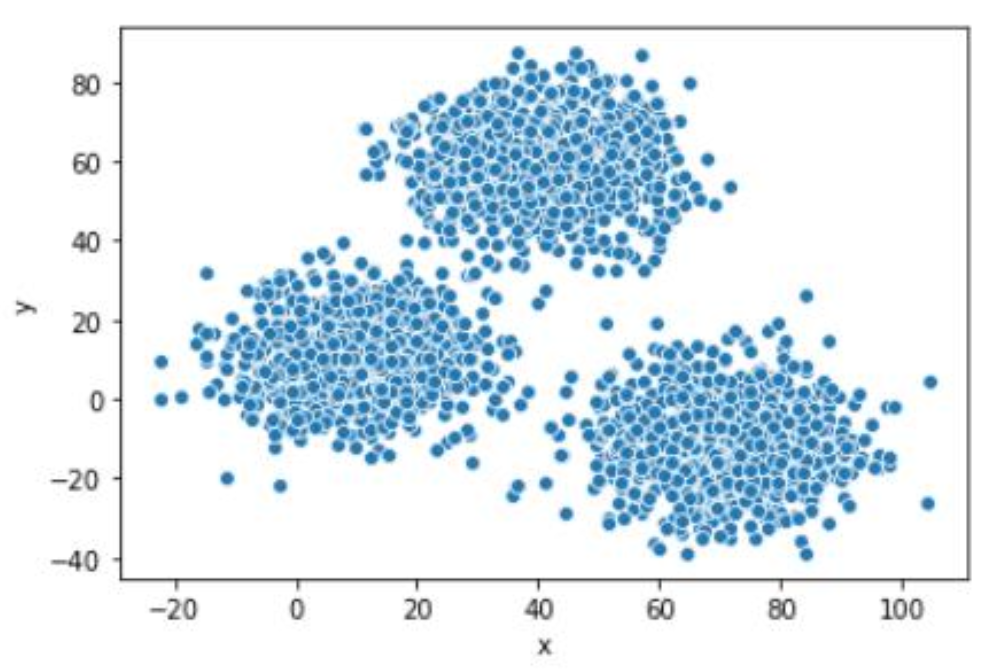
\includegraphics[scale=0.23]{prototype-based.png}
    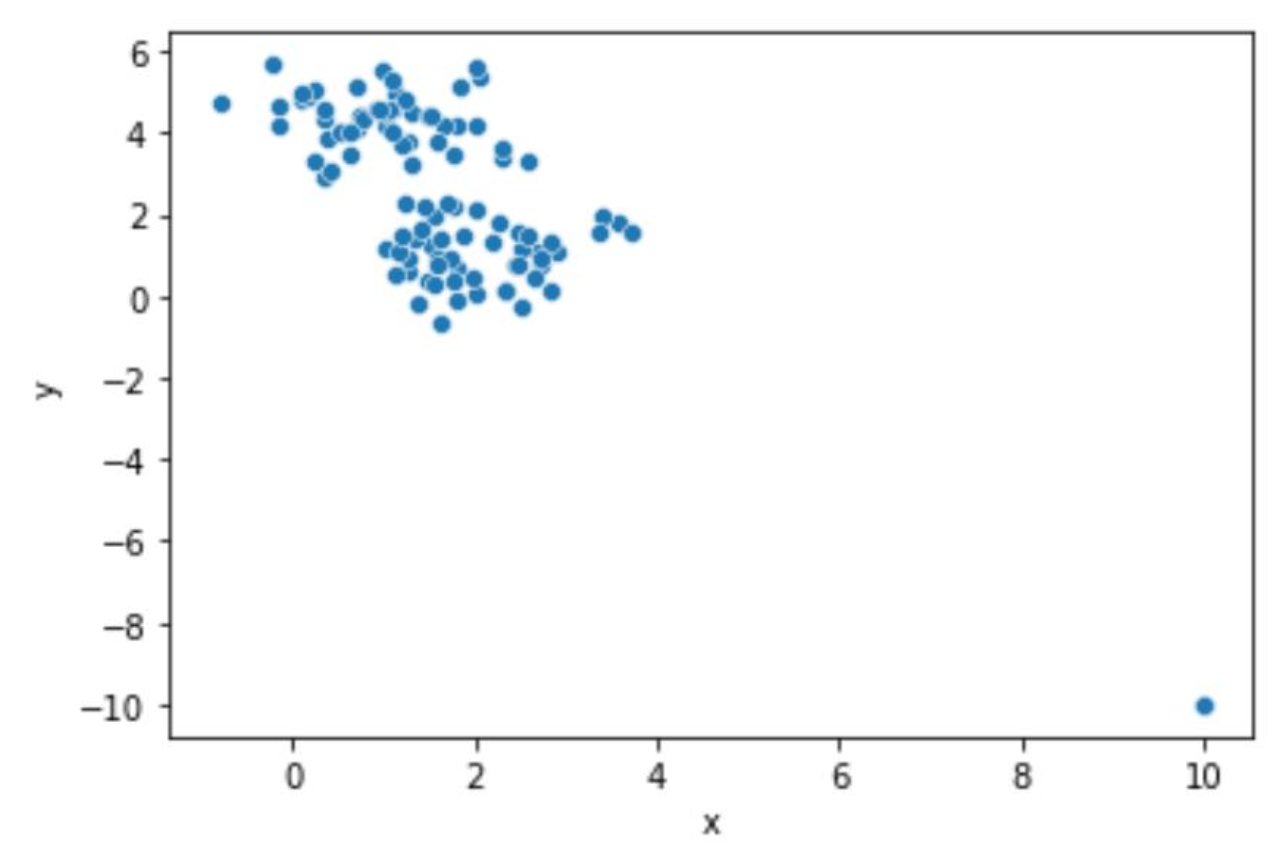
\includegraphics[scale=0.18]{prototype-based2.png}
    \caption{Prototype-Based Cluster}
\end{figure}\end{center}
\underline{Types of prototype-based clustering algorithms:}
\begin{enumerate}[$\bullet$]
    \item \textbf{K-means}: Prototype is the mean of the cluster.
    \item \textbf{K-median}: Prototype is the median of the cluster.
\end{enumerate}


\section{K-Medians}
\subsection{K-Medians Clustering Optimization Problem}

\textbf{Goal of K-Means:}

Out of all possible clustering of $\{S_1 ,S_2 , ... , S_K\}$ with $K$ clusters that can be made from the $m$ objects in $X$, find the optimal clustering $\{S_1^*,S_2^*,...,S_K^*\}$ that \underline{minimizes} the sum of the \underline{Manhattan distances} (i.e., $L_1$ distances) of each object and the centroid (the \underline{median} of the cluster that object is assigned to).

Technically, we can write this as an optimization problem
\begin{equation}
    \begin{aligned}
        \{S_1^*,S_2^*,...,S_K^*\}=\argmin_{S_1,S_2,...,S_K}\sum_{k=1}^K\sum_{x\in S_k}\|x-c_k\|_1\\
        \textnormal{Optimal Inertia}=\min_{S_1,S_2,...,S_K}\sum_{k=1}^K\sum_{x\in S_k}\|x-c_k\|_1\\
    \end{aligned}
    \nonumber
\end{equation}

\subsection{K-Medians Heuristic Algorithm}
\begin{enumerate}
    \item \textbf{Input:}
    \subitem Desired number of clusters (ex: $K=3$)
    \subitem Dataset of $m$ objects $X=\{\vec{x}_1,\vec{x}_2,...,\vec{x}_m\}$, where each object $\vec{x}_i=(x_{i1},x_{i2},...,x_{in})$ has $n$ numerical attributes. (We can also think of $X$ as being an $m\times n$ matrix $X_{m\times n}$.)
    \item \textbf{Algorithm:}
    \begin{enumerate}[$\bullet$]
        \item \textbf{\underline{Step 1:} Centroid Initialization Step}\\
        Randomly select $K$ centroids $\{\vec{c}_1,\vec{c}_2,...,\vec{c}_K\}$, where $\vec{c}_k=(c_{k1},c_{k2},...,c_{kn})$
        \item \textbf{\underline{Step 2:} Cluster Assignment Step}\\
        Assign each object $x_i$ in the dataset to its \underline{closest} centroid (specifically the \textit{smallest Manhattan distance})
        \item \textbf{\underline{Step 3:} Centroid Update Step}\\
        Find the \underline{median} of each cluster created in step 2. These medians are now the new \underline{centroids}.
        \item \textbf{\underline{Step 4:} Stopping Criterion}\\
        If the old centroids and the new centroids are the \underline{same}, stop the algorithm. Otherwise, go back to step 2.
    \end{enumerate}
    \item \textbf{Output:} Clustering with $K$ clusters $\{V_1,V_2,...,V_K\}$.
\end{enumerate}


\section{K-Medoids}
\begin{definition}[Medoid]
    In the context of clustering, we define a \textbf{medoid} as \underline{an actual object} in a cluster whose sum of distance to all the objects in the cluster is minimal.
\end{definition}
\subsection{K-Medoids Clustering Optimization Problem}

\textbf{Goal of K-Medoids:}

Out of all possible clustering of $\{S_1 ,S_2 , ... , S_K\}$ with $K$ clusters that can be made from the $m$ objects in $X$, find the optimal clustering $\{S_1^*,S_2^*,...,S_K^*\}$ that \underline{minimizes} the sum of the \underline{distances} (any distance metric) of each object and the centroid (the \underline{medoid} of the cluster that object is assigned to).

Technically, we can write this as an optimization problem
\begin{equation}
    \begin{aligned}
        \{S_1^*,S_2^*,...,S_K^*\}=\argmin_{S_1,S_2,...,S_K}\sum_{k=1}^K\sum_{x\in S_k}\textnormal{dist}(x,c_k)\\
        \textnormal{Optimal Inertia}=\min_{S_1,S_2,...,S_K}\sum_{k=1}^K\sum_{x\in S_k}\textnormal{dist}(x,c_k)\\
    \end{aligned}
    \nonumber
\end{equation}

\subsection{K-Medoids Clustering Algorithm}
\begin{enumerate}
    \item \textbf{Input:}
    \subitem Desired number of clusters (ex: $K=3$)
    \subitem Dataset of $m$ objects $X=\{\vec{x}_1,\vec{x}_2,...,\vec{x}_m\}$, where each object $\vec{x}_i=(x_{i1},x_{i2},...,x_{in})$ has $n$ numerical attributes. (We can also think of $X$ as being an $m\times n$ matrix $X_{m\times n}$.)
    \item \textbf{Algorithm:}
    \begin{enumerate}[$\bullet$]
        \item \textbf{\underline{Step 1:} Centroid Initialization Step}\\
        Randomly select $K$ centroids $\{\vec{c}_1,\vec{c}_2,...,\vec{c}_K\}$, where $\vec{c}_k=(c_{k1},c_{k2},...,c_{kn})$
        \item \textbf{\underline{Step 2:} Cluster Assignment Step}\\
        Assign each object $x_i$ in the dataset to its \underline{closest} centroid (specifically the \textit{using distance metric you've chosen})
        \item \textbf{\underline{Step 3:} Centroid Update Step}\\
        Find the \underline{medoid} of each cluster created in step 2. These medians are now the new \underline{centroids}.
        \item \textbf{\underline{Step 4:} Stopping Criterion}\\
        If the old centroids and the new centroids are the \underline{same}, stop the algorithm. Otherwise, go back to step 2.
    \end{enumerate}
    \item \textbf{Output:} Clustering with $K$ clusters $\{V_1,V_2,...,V_K\}$.
\end{enumerate}

\subsection{K-Medoids vs. K-Means}
\subsubsection*{Benefit of K-Medoids over K-Means:}
\begin{enumerate}
    \item The medoid is more robust to outliers.
    \item Guaranteed to converge using any distance metric we want (K-means has to use squared euclidean distance).
\end{enumerate}
\subsubsection*{Benefit of K-Means over K-Medoids:}
K-Medoids is more computationally complex than k-means:
\begin{enumerate}
    \item K-means: $O\left(\textnormal{number of objects}\times \textnormal{number of attributes}\times \textnormal{number of clusters}\times \textnormal{number of iterations}\right)$
    \item K-medoids: $O\left((\textnormal{number of objects})^2\times \textnormal{number of attributes}\times \textnormal{number of clusters}\times \textnormal{number of iterations}\right)$
\end{enumerate}

\section{Types of Clustering Algorithms Results}
\subsection{Partitional vs. Hierarchical Clustering Results}
\begin{definition}[Partitional Clustering]
    We call a \textbf{partitional clustering} a division of the set of data objects into $k$ subsets (clusters) such that each object is in \underline{exactly one} subset.
\end{definition}
\begin{example}
    $\{1,2,8\},\{3,7\},\{4,5,6\}$
\end{example}

\begin{definition}[Hierarchical Clustering]
    In a \textbf{hierarchical clustering} we allow for clusters to have \underline{nested subclusters}.\\
    A hierarchical
    clustering is displayed as a set of nested clusters displayed as a \textbf{dendrogram} tree. The dendrogram can reflect which objects and clusters are closer to each other than others.
\end{definition}
\begin{example}
    $\{\{1,3\},\{\{\{6,9\},10\},\{11,15\}\}\},\{4,\{12,19\}\},\{\{\{2,14\},\{\{17,20\},18\}\},\{5,8\}\},\{7,\{13,16\}\}$.
\end{example}
\begin{center}\begin{figure}[htbp]
    \centering
    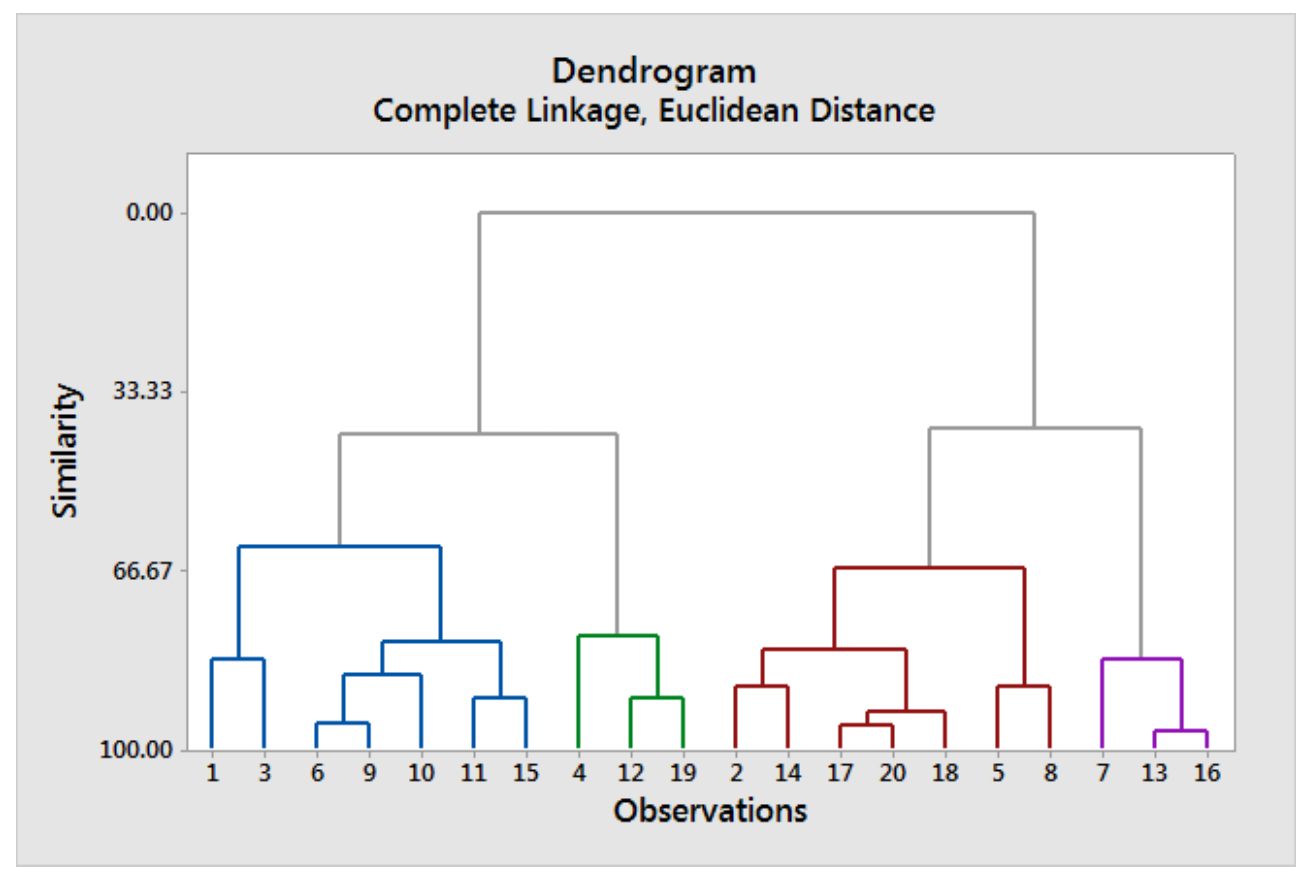
\includegraphics[scale=0.25]{Hierarchical Clustering.png}
    \caption{Hierarchical Clustering Example}
    \label{}
\end{figure}\end{center}

\subsection{Exclusive vs. Overlapping vs. Fuzzy Clustering Results}
\begin{definition}
    \textbf{Exclusive Clustering} will assign an object to an \underline{exactly one cluster}.
\end{definition}
\begin{example}
    $\{1,3,5\},\{2,4\}$.
\end{example}
\begin{definition}
    \textbf{Overlapping Clustering} can allow for an object to be assigned to \underline{more than one cluster}.
\end{definition}
\begin{example}
    $\{1,3,5\},\{2,4,5\}$
\end{example}

\begin{definition}
    In a \textbf{Fuzzy Clustering} every object belongs to every cluster with a membership weight that is between $0$ (absolutely doesn't belong to the cluster) to $1$ (absolutely belongs).
    \begin{enumerate}
        \item Usually the sum of each object's weights must sum to $1$.
        \item $w_{ij}$ $=$ the probability that object $i$ belongs to cluster $j$.
    \end{enumerate}
\end{definition}








\chapter{Clustering Evaluation Metrics}
\begin{center}\begin{figure}[htbp]
    \centering
    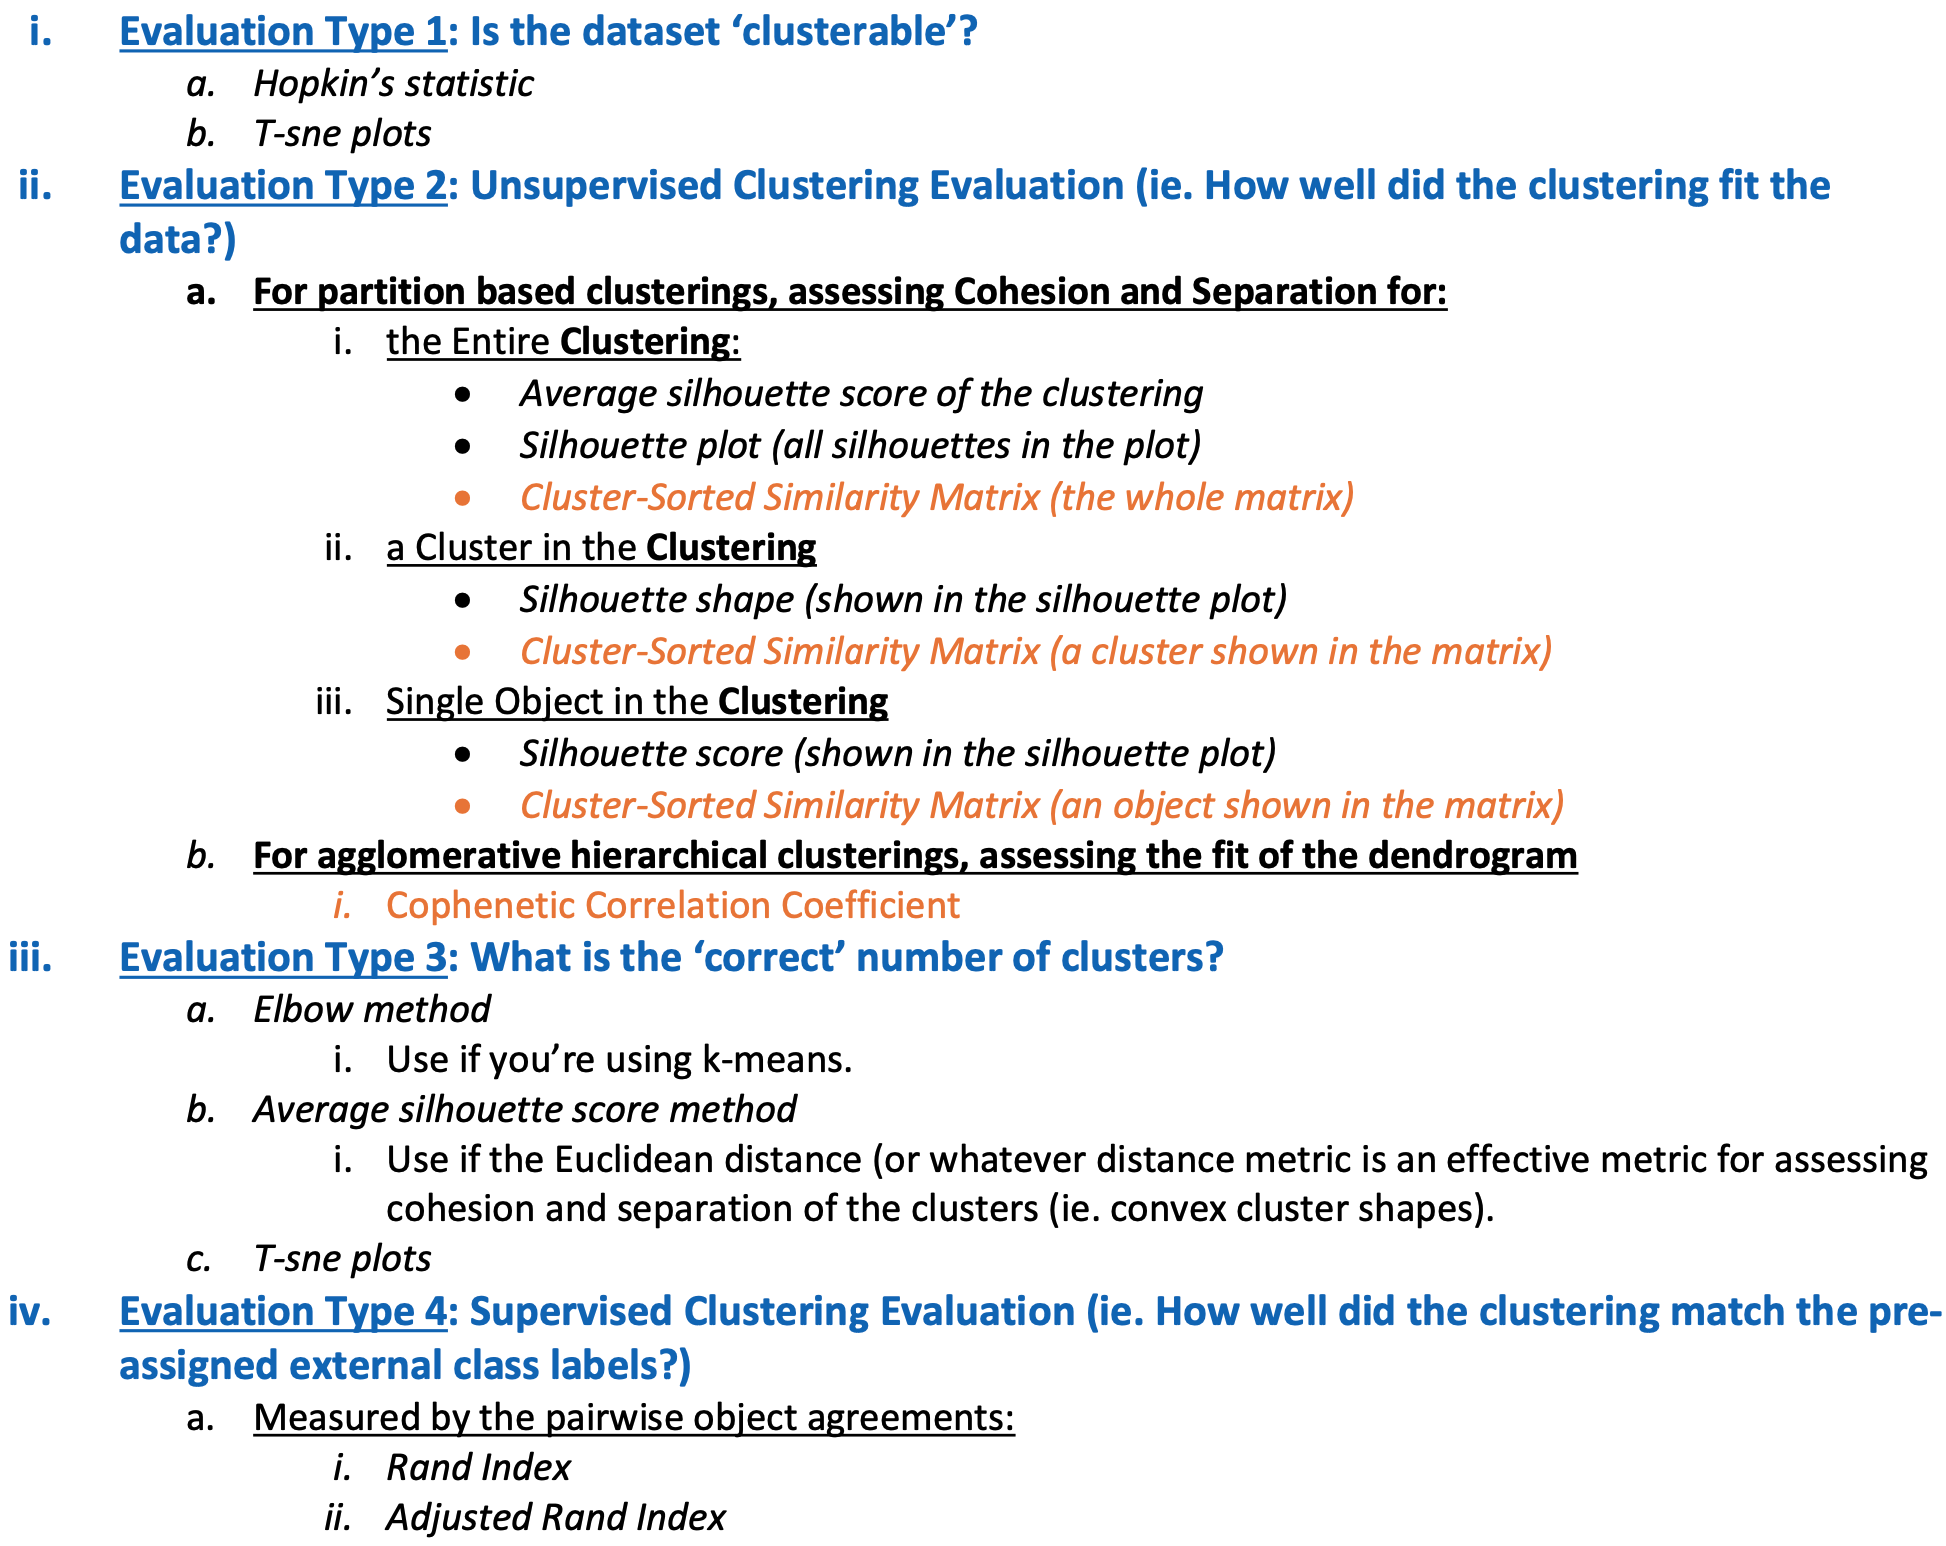
\includegraphics[scale=0.23]{metric1.png}
    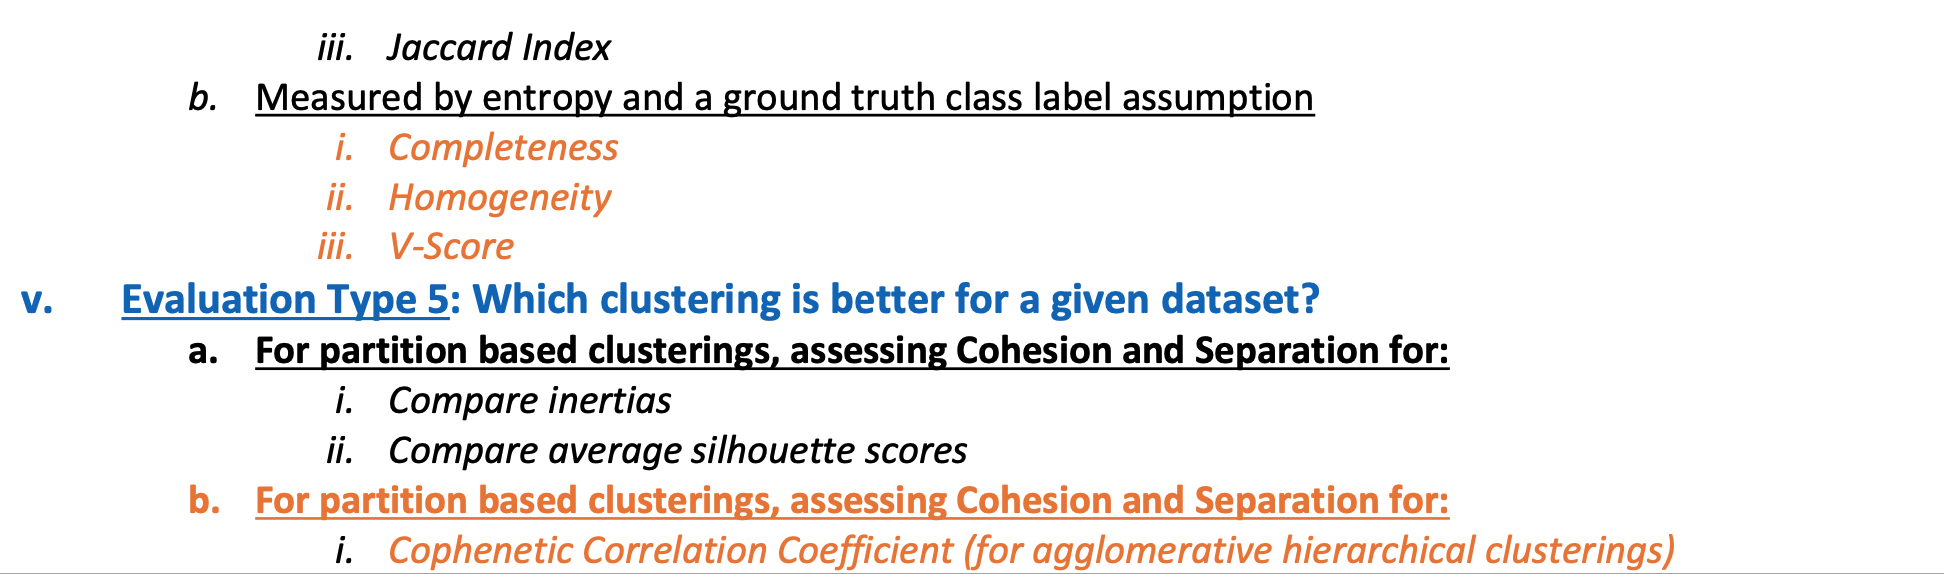
\includegraphics[scale=0.23]{metric2.png}
    \caption{Evaluation Metrics}
    \label{}
\end{figure}\end{center}





\section{Clusterability Evaluation Metric: Is the dataset clusterable?}
\begin{definition}
    A dataset is \textbf{clusterable} if there exist some distinct groupings of observations in a dataset.
\end{definition}
Then, how distinct do the observation need to be is a question.


\subsection{Hopkin's Statistics}
\begin{enumerate}[$\bullet$]
    \item \textbf{\underline{Input:}} Dataset of $m$ objects $X=\{\vec{x}_1,\vec{x}_2,...,\vec{x}_m\}$, where each object $\vec{x}_i=(x_{i1},x_{i2},...,x_{in})$ has $n$ numerical attributes.
    \item \textbf{\underline{How to calculate:}}
    \begin{enumerate}[$(1)$]
        \item Create a set of random \underline{artificial data point} closest distances $\{u_1,u_2,...,u_p\}$ as follows.
        \begin{enumerate}[a)]
            \item Generate $p$ \underline{random artificial data points} $\{\vec{y}_1, \vec{y}_2, ... , \vec{y}_p\}$ distributed across
            the range of the dataset.
            \item For each random artificial data points $i=1,...,p$ calculate $$u_i=\min_{\vec{x}\in X}\textnormal{dist}(\vec{y}_i,\vec{x})$$
        \end{enumerate}
        \item Create a set of random \underline{actual data point} closest distances $\{w_1,w_2,...,w_p\}$ as follows.
        \begin{enumerate}[a)]
            \item Random select $p$ \underline{actual points} $\{\vec{z}_1, \vec{z}_2, ... , \vec{z}_p\}$ from the dataset.
            \item For each randomly selected actual points $i=1,...,p$ calculate $$w_i=\min_{\vec{x}\in X}\textnormal{dist}(\vec{z}_i,\vec{x})$$
        \end{enumerate}
        \item $$\textbf{Hopkins Statistic}=\frac{\sum_{i=1}^p w_i}{\sum_{i=1}^p w_i+\sum_{i=1}^p u_i}$$
    \end{enumerate}
    \item \textbf{\underline{How to interpret:}} The dataset is \underline{clusterable} if the Hopkins Statistic \underline{close to $0$} and is \underline{not clusterable} if the Hopkins Statistic \underline{close to $0.5$}.
    \item \textbf{\underline{Intuition:}}
    \begin{center}\begin{figure}[htbp]
        \centering
        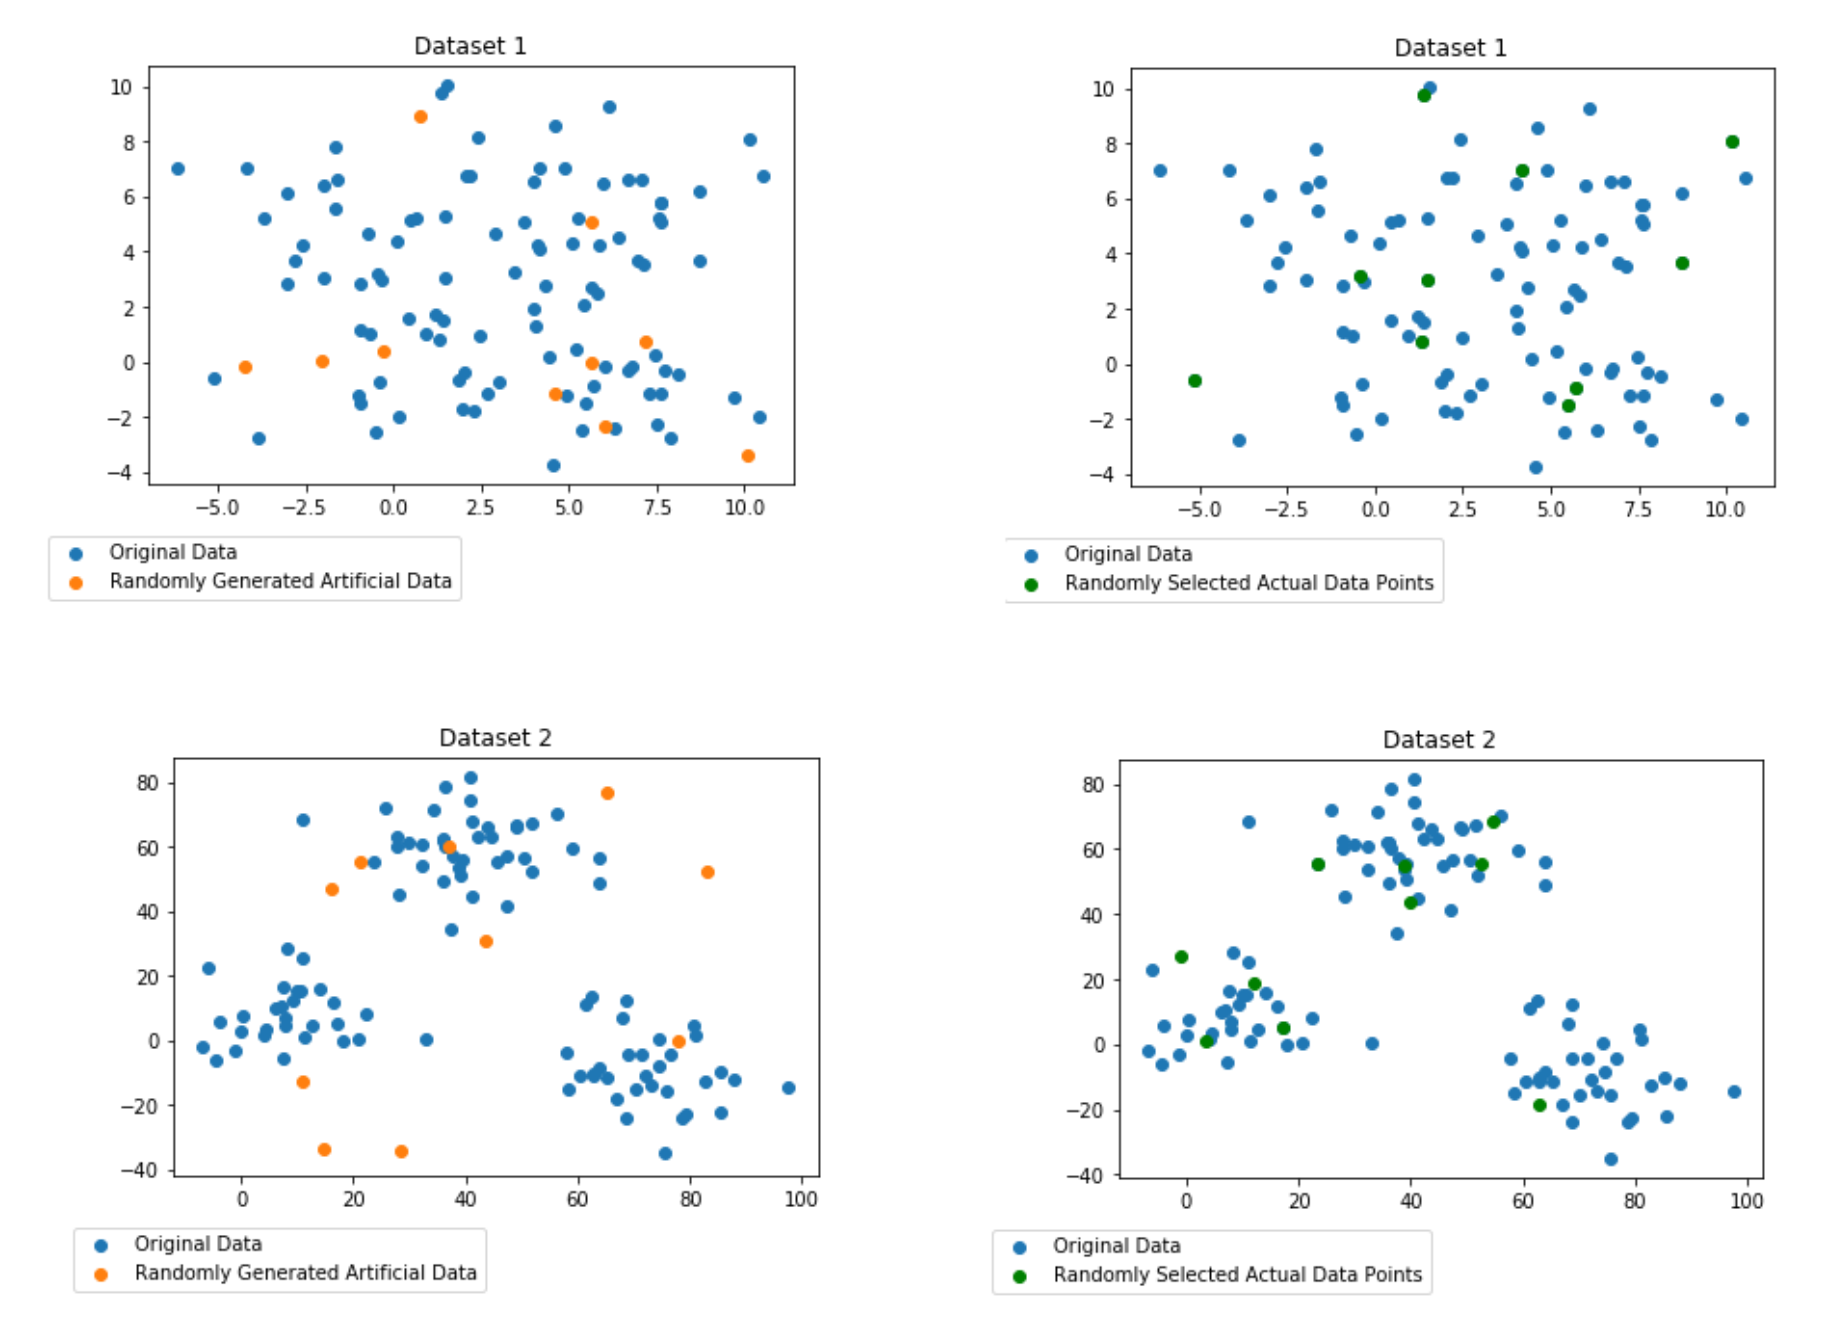
\includegraphics[scale=0.25]{HS.png}
        \caption{When Hopkins Statistic works well and not well}
        \label{}
    \end{figure}\end{center}
    \item \textbf{\underline{Additional Tips and Information:}} $p=10\%\times \textnormal{(the number of observations in the dataset)}$; Hopkins Statistic is \underline{non-deterministic} evaluation metric.
\end{enumerate}

\section{Unsupervised Clustering Evaluation Metrics: How cohesive and well separated are the clusters in the
clustering?}
\subsection{Definition}
\begin{definition}
    \textbf{Unsupervised clustering evaluation metrics} evaluate the goodness of the clustering without using pre-assigned class labels.
\end{definition}

\underline{Types of Unsupervised Clustering Evaluation Metrics:}
\begin{enumerate}
    \item \textbf{Cohesion} measures how closely related the objects in a cluster are.
    \item \textbf{Separation} measures how distinct or well-separated a cluster is from other clusters.
    \item \textbf{Validity of a clustering} can be expressed as some function of \textbf{cohesion} and \textbf{separation} of all the clusters in a clustering.
\end{enumerate}

\subsection{Graph-based view of cohesion and separation for a clustering}
A graph-based view of calculating cohesion and separation for a clustering involves first creating a \textbf{proximity matrix} (graph) of the objects in the dataset, that measures the “proximity” of each pair of objects in the dataset.
\begin{center}\begin{figure}[htbp]
    \centering
    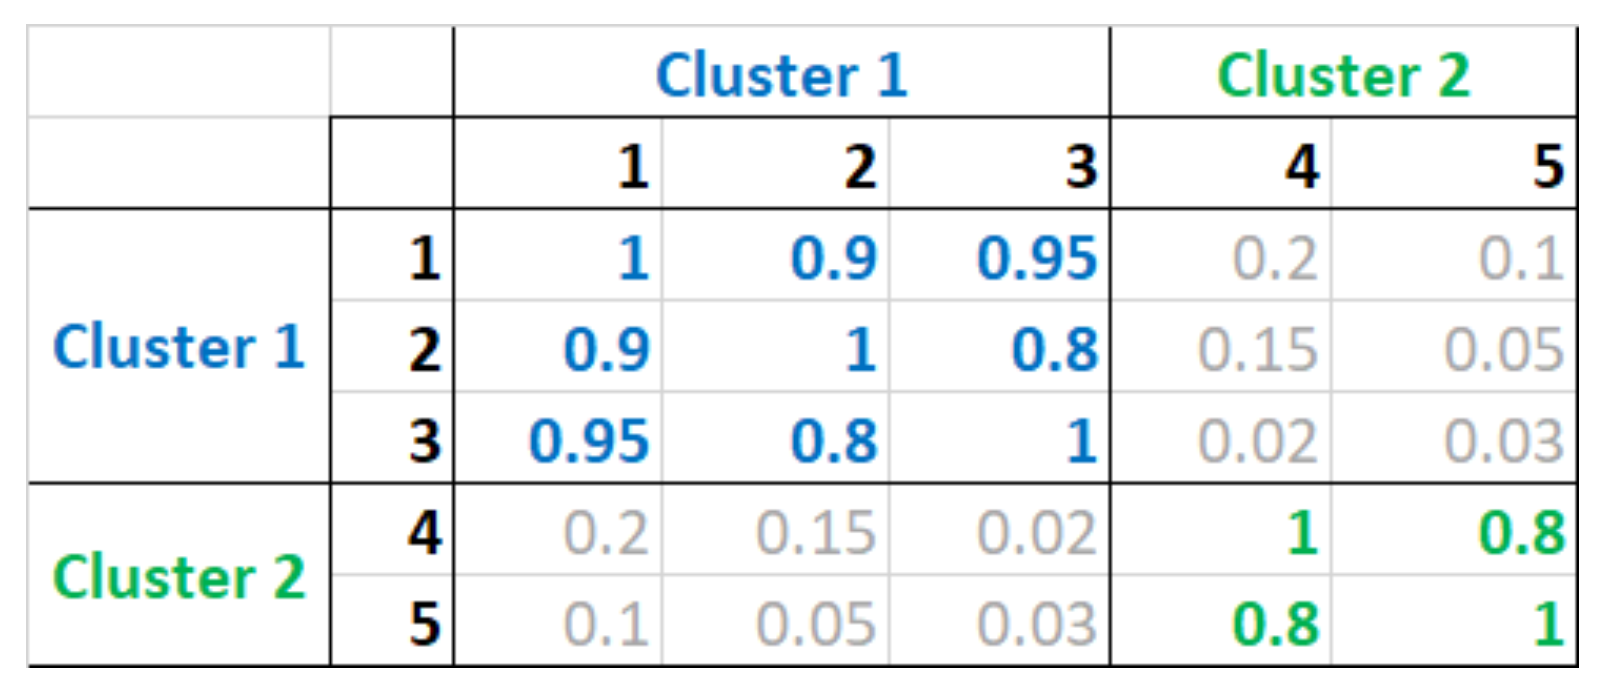
\includegraphics[scale=0.18]{proximity matrix.png}
    \caption{Proximity Matrix}
    \label{}
\end{figure}\end{center}
\underline{Different ways to measure proximity:}
\begin{enumerate}
    \item \textbf{Similarity metric measure of proximity:} The more similar two objects are the lower the proximity measure is. e.g. Euclidean distance.
    \item \textbf{Dissimilarity metric measure of proximity:} The more similar two objects are the higher this proximity measure is. e.g. The number of attribute agreements between two categorical objects.
\end{enumerate}

\underline{\textbf{Cohesion} of a graph-based cluster} is the sum of proximities between all pairs of points within the same cluster.
\begin{equation}
    \begin{aligned}
        \textnormal{cohesion}(C_i)=\sum_{\vec{x}\in C_i,\vec{y}\in C_i}\textnormal{proximity}(\vec{x},\vec{y})
    \end{aligned}
    \nonumber
\end{equation}

\underline{\textbf{Separation} of a graph-based cluster} is the sum of proximities between all pairs of points in the two different clusters.
\begin{equation}
    \begin{aligned}
        \textnormal{separation}(C_i,C_j)=\sum_{\vec{x}\in C_i,\vec{y}\in C_j}\textnormal{proximity}(\vec{x},\vec{y})
    \end{aligned}
    \nonumber
\end{equation}

\subsection{Silhouette Coefficients (Scores)}
\begin{enumerate}
    \item \textbf{Cohesion Metric:} Measure of how “well assigned” object $x_i$ is to cluster $C_k$: $$a_i=\frac{1}{|C_k|-1}\sum_{\vec{x}_j\in C_k,\vec{x}_i\neq \vec{x}_j}\textnormal{dist}(\vec{x}_i,\vec{x}_j)$$
    \item \textbf{Separation Metric:} Find the Average Distance of object $x_i$ to it's "neighboring cluster." $$b_i=\min_{k'\neq k}\frac{1}{|C_{k'}|}\sum_{\vec{x}_j\in C_{k'}}\textnormal{dist}(\vec{x}_i,\vec{x}_j)$$
    \item \textbf{Silhouette Coefficient (Score)} of $x_i$
    $$s_i=\left\{\begin{matrix}
        \frac{b_i-a_i}{\max\{a_i,b_i\}},&\textnormal{if }|C_i|>1\\
        0,&\textnormal{if }|C_i|=1
    \end{matrix}\right.$$
\end{enumerate}
The silhouette of a cluster visualizes the silhouette values $s_i$ of all the points in it in the \underline{decreasing order}. A silhouette plot shows the silhouettes of all the clusters in random order. Additionally, it inserts blank spaces between consecutive clusters and can color them differently.
\begin{center}\begin{figure}[htbp]
    \centering
    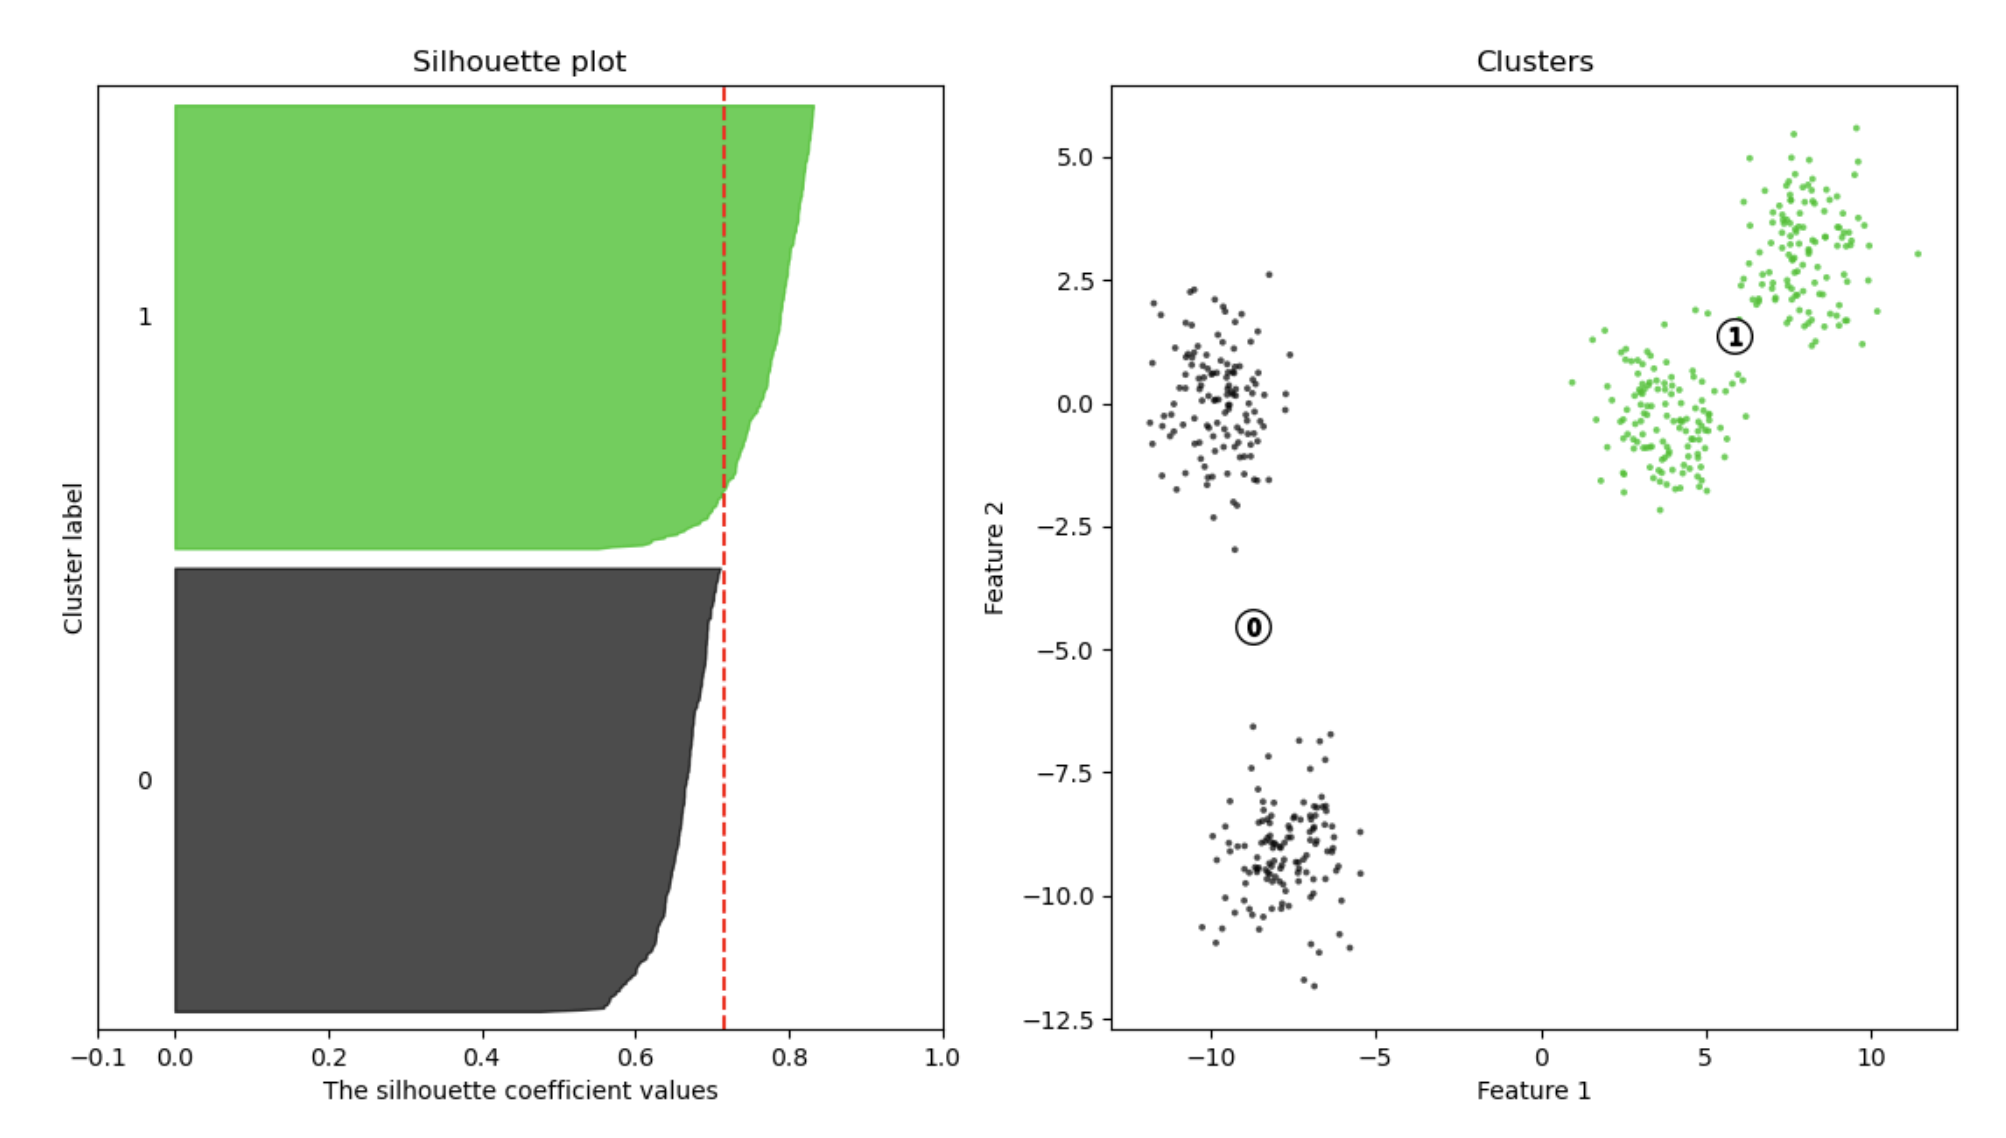
\includegraphics[scale=0.2]{Silhouette Plots.png}
    \caption{Silhouette Plots}
    \label{}
\end{figure}\end{center}

\begin{enumerate}
    \item \textbf{Silhouette Coefficient} $s_i$ of object $\vec{x}_i$ is \underline{large and positive}: the object is \underline{closer} to objects in the cluster that it is assigned to than objects in other clusters.
    \item \textbf{Silhouette Coefficient} $s_i$ of object $\vec{x}_i$ is \underline{close to $0$}: the object is \underline{equally close} to objects in the cluster that it is assigned to than objects in other clusters.
    \item \textbf{Silhouette Coefficient} $s_i$ of object $\vec{x}_i$ is \underline{large and negative}: the object is \underline{further away from} to objects in the cluster that it is assigned to than objects in other clusters.
\end{enumerate}
\textbf{Warning:} Silhouette coefficients and plots (based off of Euclidean distances) will not be effective at assessing clustering separation and cohesion for all types of datasets. (e.g. the contiguity-based cluster.) We need to revise the distance metric.

\subsection{Prototype-Based View of Cohesion and Separation for a Clustering}
\begin{enumerate}
    \item \textbf{Cohesion of a prototype-based cluster:} the sum of proximities between all points \underline{in a given cluster} and the \underline{prototype} of that cluster.
    \item \textbf{Separation of a prototype-based cluster:} the proximity of the two cluster prototypes.
\end{enumerate}

\subsection{Cluster-Sorted Similarity Matrix}
How to Create: The Cluster-Sorted Similarity (or Distance) Matrix of the Partition-Based Clustering
\begin{enumerate}[$\bullet$]
    \item Step 1: Sort the dataset by the cluster labels that have been assigned to each object.
    \item Step 2: Keeping the new order (giving the objects new indices), create a pairwise-distance matrix $\left[\textnormal{dist}_{ij}\right]$ between all objects and visualize it. (not with the cluster labels)
    \item Step 3 (optional): Keep a mapping from the old object indices to the new object indices.
\end{enumerate}
\begin{center}\begin{figure}[htbp]
    \centering
    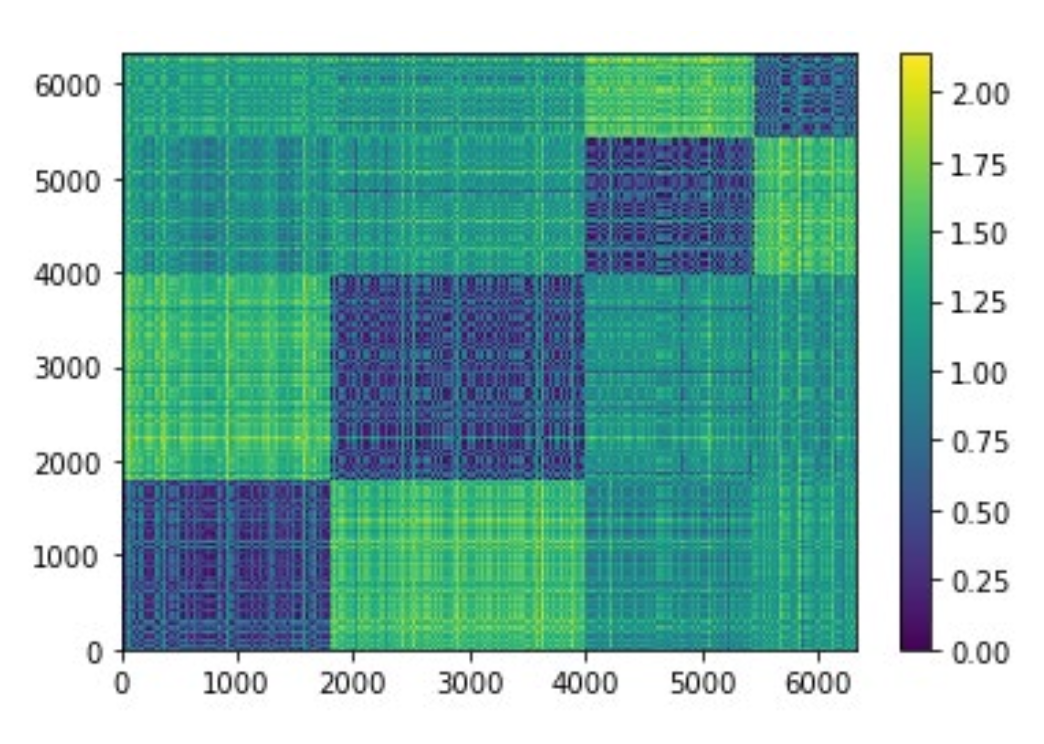
\includegraphics[scale=0.25]{CSSM.png}
    \caption{Example of Cluster-Sorted Similarity Matrix}
    \label{}
\end{figure}\end{center}
\textbf{Limitations}: This method (if you plan to use the euclidean distance metric) is not as useful at evaluating the cohesion and separation of non-convex clusters.



\section{Cluster Number Evaluation Metrics: What is the 'correct' number of clusters?}

\subsection{General Elbow Plot Method}
\begin{definition}[General Elbow Plot Method]
    When determining whether a clustering structure can be detected by a particular clustering algorithm (K-means, K-medians, K-medoids), we can use an elbow plot that plots the value of the objective function that we are trying to minimize of the clusterings found by that particular clustering algorithm with $k=1,k=2,...$ clusters respectively.
\end{definition}

The \textbf{drawback} of this method is each of these methods are dependent on the ability of a clustering algorithm to detect the clustering structure.

\subsection{Average Silhouette Score Plot Method}
\begin{enumerate}[(1).]
    \item \textbf{\underline{Creating an Average Silhouette Score Plot}}\\
    For $k=1$ to $K$:
    \begin{enumerate}[$\bullet$]
        \item Cluster the data several times into k clusters.
        \item Calculate the average of the average silhouette scores of these resulting
        clusterings.
        \item Then plot the average of these average silhouette scores for each $k$.
    \end{enumerate}
    \begin{center}\begin{figure}[htbp]
        \centering
        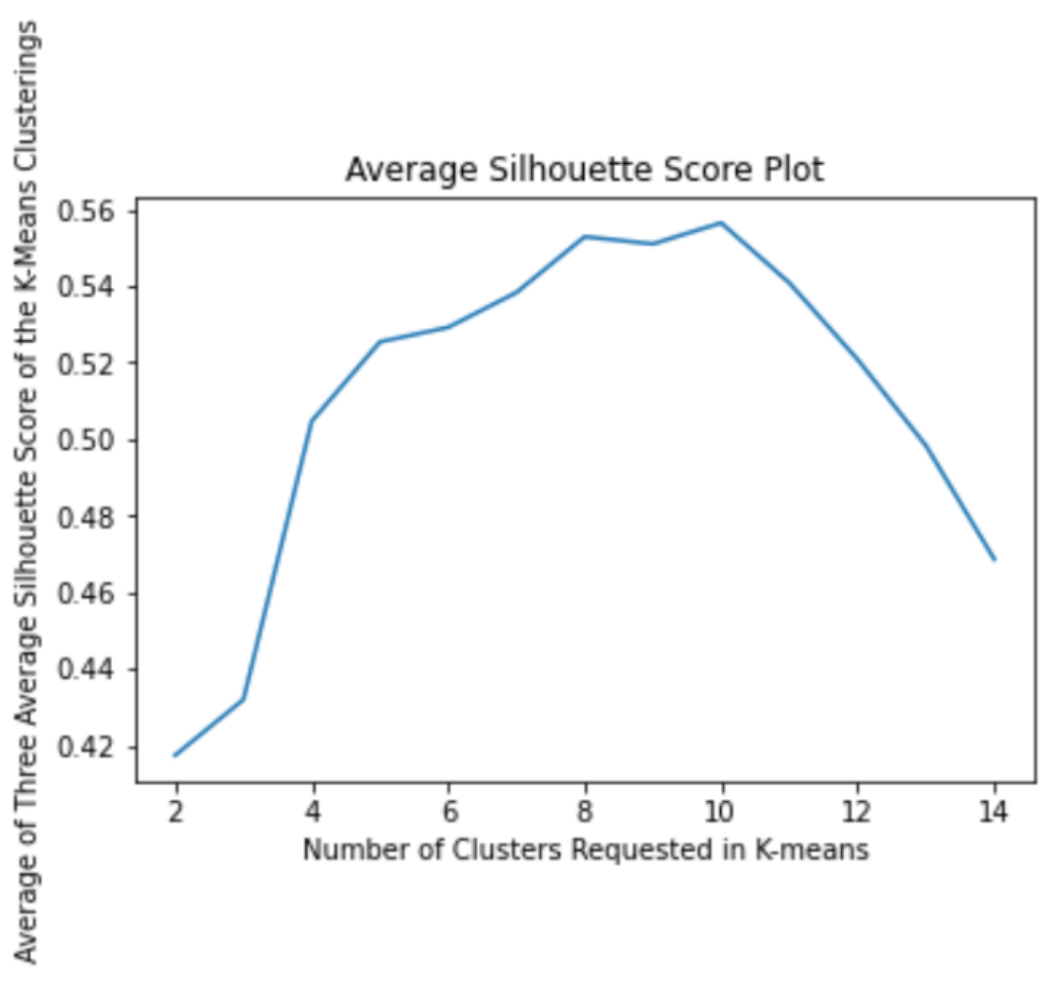
\includegraphics[scale=0.2]{Average Silhouette Score Plot.png}
        \caption{Average Silhouette Score Plot}
        \label{}
    \end{figure}\end{center}
    \item \textbf{\underline{How to interpret:}} Choose the number of clusters with the highest average silhouette score.
    \item \textbf{\underline{Warning:}} We need to make sure the distance metric we are using to measure the silhouette score with is a useful metric in measuring the cohesion and the separation of
    the clusters in the dataset.\\
    For instance, when using the Euclidean distance to measure distance in the silhouette score, the average silhouette score is not as effective in measuring clustering cohesion and separation of \textbf{non-convex shapes}.
    \item \textbf{\underline{Benefit:}} Using an average silhouette score plot do not assume using one particular algorithm/clustering problem to measure cluster performance.
\end{enumerate}




\section{Supervised Clustering Evaluation Metrics: How similar is the clustering to a set of (external) pre-assigned class labels?}

\begin{definition}[Supervised Clustering Evaluation Metrics]
    \textbf{Supervised clustering evaluation metrics} evaluate the clustering by using a set of pre-assigned class labels. This can be useful for examining the association between our pre-assigned cluster labels and the clustering structure identified by our clustering algorithms.
\end{definition}

\subsection{Rand Index and Jaccard Coefficient of Two Partitions}
A partition of a set $\{x_1, x_2, ... , x_m\}$ is a collection of $K$ non-empty subsets (i.e. clusters/classes) of the set such that every element of the set is in exactly one of the subsets (i.e. clusters/classes).
\begin{definition}[Rand Index and Jaccard Coefficient]
    \begin{equation}
        \begin{aligned}
            \textnormal{Rand Index (Statistic)}&=\frac{f_{00}+f_{11}}{f_{00}+f_{01}+f_{10}+f_{11}}\\
            \textnormal{Jaccard Coefficient}&=\frac{f_{11}}{f_{01}+f_{10}+f_{11}}\\
        \end{aligned}
        \nonumber
    \end{equation}
    \begin{enumerate}[$\circ$]
        \item $f_{00}=$ number of pairs of objects in the dataset that are \textbf{apart} in partition 1 and partition 2
        \item $f_{11}=$ number of pairs of objects in the dataset that are \textbf{together} in partition 1 and partition 2
        \item $f_{01}=$ number of pairs of objects in the dataset that are \textbf{apart} in partition 1 and \textbf{together} in partition 2
        \item $f_{10}=$ number of pairs of objects in the dataset that are \textbf{together} in partition 1 and \textbf{apart} in partition 2
    \end{enumerate}
\end{definition}
\textbf{Interpretation and Ranges:}
\begin{enumerate}
    \item Rand Index (Statistic)$\in [0,1]$: $0$ means all possible object pairs disagree between the two partitions; $1$ means the partitions are exactly the same.
    \item Jaccard Coefficient$\in [0,1]$: $0$ means none of the possible object pairs that have
    at least one partition
    that has put them
    together are together in both partitions; $1$ means all possible object pairs that have at least one partition that has put them together are together in both partitions.
\end{enumerate}

\subsection{Adjusted Rand Index}
In Rand Index (Statistic), $0$ means all possible object pairs disagree between the two partitions and $1$ means clusterings are identical. However, we want a desired evaluation metric such that, $0$ means random labeling independently of the number of clusters and samples and $1$ means clusterings are identical

\begin{definition}[Adjusted Rand Index]
    \begin{equation}
        \begin{aligned}
            \textnormal{Adjusted Rand Index}=\frac{\textnormal{rand index}-\textnormal{expected rand index}}{\textnormal{maximum rand index}-\textnormal{expected rand index}}
        \end{aligned}
        \nonumber
    \end{equation}
\end{definition}
For two partitions $\{U_1,U_2,...,U_K\}$ and $\{V_1,V_2,...,V_{K'}\}$ of the same set of $m$ objects, we can define:
\begin{enumerate}
    \item $m_{k,k'}=$number of objects in common in subset $U_k$ and $V_{k'}$.
    \item $a_k=$the total number objects in subset $U_k$.
    \item $b_{k'}=$the total number objects in subset $V_{k'}$.
\end{enumerate}
\begin{equation}
    \begin{aligned}
        \textnormal{Adjusted Rand Index}=\frac{\sum_{k,k'}\begin{pmatrix}
            m_{k,k'}\\
            2
        \end{pmatrix}-\left[\sum_k\begin{pmatrix}
            a_{k}\\
            2
        \end{pmatrix}\sum_{k'}\begin{pmatrix}
            b_{k'}\\
            2
        \end{pmatrix}\right]/\begin{pmatrix}
            m\\
            2
        \end{pmatrix}}{\frac{1}{2}\left[\sum_k\begin{pmatrix}
            a_{k}\\
            2
        \end{pmatrix}+\sum_{k'}\begin{pmatrix}
            b_{k'}\\
            2
        \end{pmatrix}\right]-\left[\sum_k\begin{pmatrix}
            a_{k}\\
            2
        \end{pmatrix}\sum_{k'}\begin{pmatrix}
            b_{k'}\\
            2
        \end{pmatrix}\right]/\begin{pmatrix}
            m\\
            2
        \end{pmatrix}}
    \end{aligned}
    \nonumber
\end{equation}
Adjusted rand index can actually be negative for two clusterings that have very low similarity.








\section{Clustering Comparison Metrics: Which clustering is better for a given dataset?}
\begin{enumerate}
    \item \textbf{Inertias} of the two clusterings:    Inertia should only be used to compare clustering generated from the \textbf{same dataset}.
    \item \textbf{Average silhouette scores} of the two clusterings: We can use this metric to compare the cohesion and separation of clusterings (and they \textbf{could} be two clusterings of \textbf{different dataset}),
\end{enumerate}


\section{'Clusterable'?  and 'Correct' Number of Clusters: $t$-SNE}
$t$-SNE is $t$-Distributed Stochastic Neighbor Embedding

We want to use $t$-SNE plots help us visualize some aspects of the underlying clustering structure of the data.

\subsection{Goal}
\textbf{\underline{Goal}}: project multidimensional data onto a $2$ or $3$-dimensional plane while preserving \textbf{clustering structure} of the dataset.

We want to use $t$-SNE plots help us visualize some aspects of the underlying clustering structure of the data:
\begin{enumerate}
    \item Whether there \underline{exists} a \textbf{clustering structure} in the data.
    \item Approximation of the \textbf{number of clusters}.
    \item Approximation of the \textbf{cluster shapes}.
    \item Approximate \textbf{number of objects} in each cluster.
    \item Approximation of whether clusters are
    \textbf{separated} or not.
    \item Approximation how any \textbf{pre-assigned class labels} \underline{associate} with the underlying \textbf{clustering structure of the data}.
    \item Approximation of how any \textbf{cluster labels (from a clustering algorithm)} associate with the \textbf{underlying clustering structure of the data suggested by the t-SNE algorithm}.
\end{enumerate}

\subsection{Input/Output for the Algorithm}
\textbf{Input:}
\begin{enumerate}[$\bullet$]
    \item \underline{Dataset} of $m$ objects $X=\{\vec{x}_1,\vec{x}_2,...,\vec{x}_m\}$, where each object $\vec{x}_i=(x_{i1},x_{i2},...,x_{in})$ has $n$ numerical attributes.
    \item \underline{Number of Dimensions:} Dimension of the data you want to project the data onto (usually 2).
    \item \underline{Number of Iterations:} maximum number of iterations for the algorithm.\\
    \textit{How to select:} (1). At least 200; (2). Automatically set to 1000 in Python (which tends to work for many, but not all datasets); (3). Keep iterating until you see a stable configuration of the shapes.
    \item \underline{Perplexity}, which says (loosely) how to balance attention between local and global aspects of your data. The parameter is, in a sense, a guess about the number of close neighbors each point has.\\
    \textit{How to select:} (1). Works best when $5 \leq$ perplexity $\leq 50$; (2). Perplexity $<$ \underline{number of objects}.
\end{enumerate}
\begin{center}\begin{figure}[htbp]
    \centering
    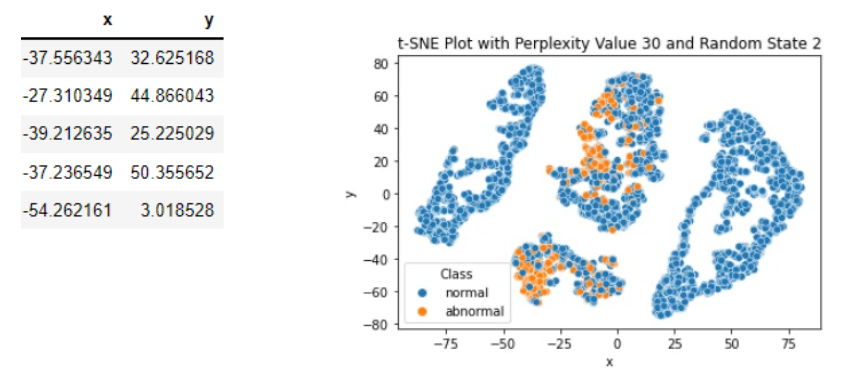
\includegraphics[scale=0.5]{tsne_example_of_output.png}
    \caption{Example of Output}
    \label{}
\end{figure}\end{center}

\subsection{Main Idea of The Algorithm}
\begin{enumerate}
    \item \textbf{\underline{Optimization Problem:}} Given an original high dimensional dataset, we need to solve an optimization for the optimal value of the decision variables that represent the low-dimensional projected coordinates for each observation in the original dataset.\\
    $\vec{x}_i=[x_{1,1},...,x_{1,n}] \Rightarrow \vec{y}_i=[y_{i,1},y_{i,2}],\ i=1,2...,m$.
    \begin{center}\begin{figure}[htbp]
        \centering
        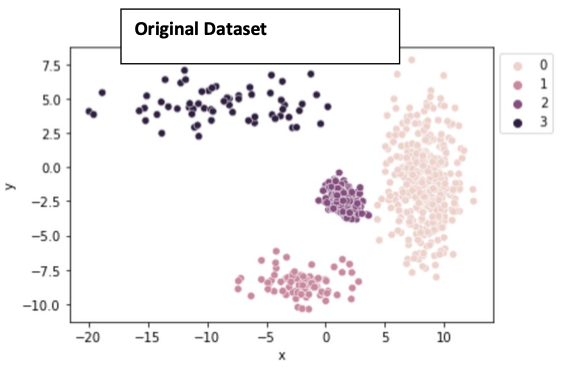
\includegraphics[scale=0.4]{OP_tsne.png}
        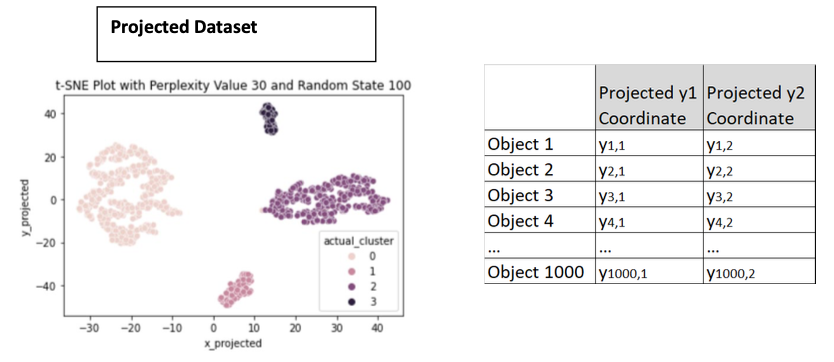
\includegraphics[scale=0.4]{OP_tsne_2.png}
        \caption{Optimization Problem}
        \label{}
    \end{figure}\end{center}
    \item \textbf{\underline{Crates a Similarity matrix $P$ for the Points in the Original Dataset:}}
    Similarity between a given point $\vec{x}_i$ and another point $\vec{x}_j$ is a function of a normal distribution centered at $\vec{x}_i$ with a standard deviation $\sigma_i$ that changes based on the point and how many "neighbors" you think each point in the dataset has. Each entry of the matrix is the \textbf{similarity} between $i$ and $j$.
    \begin{equation}
        \begin{aligned}
        p_{i j}= & \frac{1}{2m}\left(p_{j \mid i}+p_{i \mid j}\right) \\
        & \bullet p_{j \mid i}=\frac{\exp \left(-\frac{\left\|\vec{x}_i-\vec{x}_j\right\|^2}{2 \sigma_i^2}\right)}{\sum_{k \neq i} \exp \left(-\frac{\left\|\vec{x}_i-\vec{x}_k\right\|^2}{2 \sigma_i^2}\right)} \\
        & \bullet p_{i \mid j}=\frac{\exp \left(-\frac{\left\|\vec{x}_i-\vec{x}_j\right\|^2}{2 \sigma_j^2}\right)}{\sum_{k \neq j} \exp \left(-\frac{\left\|\vec{x}_j-\vec{x}_k\right\|^2}{2 \sigma_j^2}\right)}
        \end{aligned}
        \nonumber
    \end{equation}
    \item \textbf{\underline{Creates a Similarity Matrix $Q$ for the Points (i.e., Decision Variables we are Trying to Solve for)} in the \underline{Projected Dataset}:} Similarity between a given point $\vec{y}_i$ and another point $\vec{y}_j$ is a function about $t$-distribution centered at $\vec{y}_i$.
    $$q_{ij}=\frac{(1+\|\vec{y}_i-\vec{y}_j\|^2)^{-1}}{\sum_{k\neq l}(1+\|\vec{y}_k-\vec{y}_j\|^2)^{-1}}$$
    \item Solve the optimization problem:
    \begin{equation}
        \begin{aligned}
            \min_{\{\vec{y}_i\}_{i=1}^m}\textnormal{dist}(P,Q)=D_{KL}(P\| Q)=\sum_i\sum_j p_{ij}\log\frac{p_{ij}}{q_{ij}}
        \end{aligned}
        \nonumber
    \end{equation}
    A heuristic solution to this optimization problem can be found via a \underline{Gradient Descent algorithm}.
\end{enumerate}


Algorithm is heavy on both time and space resources $O(n^2)$. Computationally ineffective for datasets with more than $10000$ observations.

\chapter{Hierarchical Clustering}
\section{Agglomerative and Divisive Hierarchical Clustering Algorithms}
\textbf{Hierarchical clustering algorithms} allow us to display a series of nested clusterings, graphically displayed in a dendrogram.
\begin{center}\begin{figure}[htbp]
    \centering
    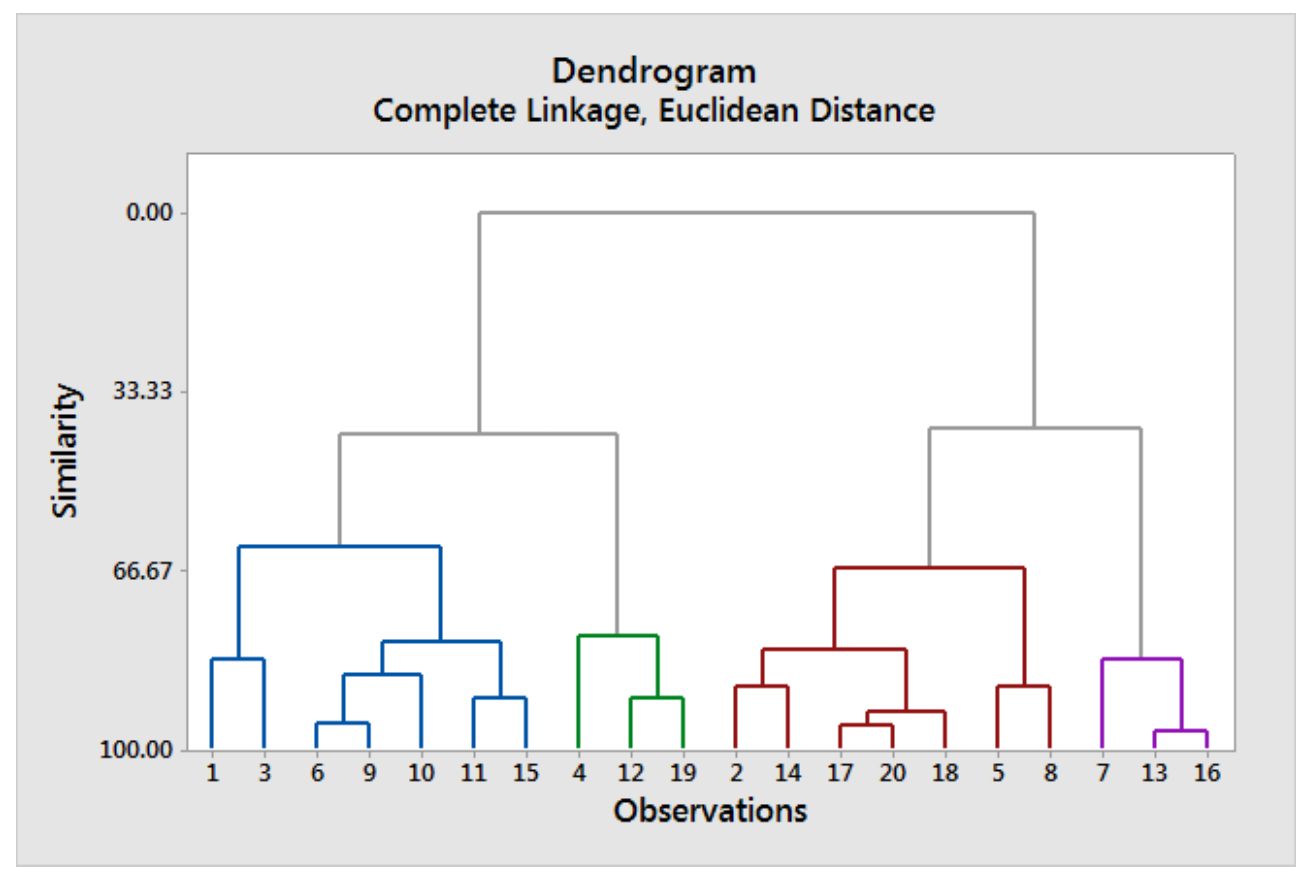
\includegraphics[scale=0.2]{Hierarchical Clustering.png}
    \caption{Hierarchical Clustering Example}
    \label{}
\end{figure}\end{center}

\begin{enumerate}
    \item An \textbf{\underline{ agglomerative hierarchical clustering algorithm}} starts with all objects \textbf{apart in singleton clusters} and then iteratively joins clusters together until all objects
    are in the same cluster.
    \item A \textbf{\underline{ divisive hierarchical clustering algorithm}} starts with all objects \textbf{together} and then iteratively divides clusters together until all objects
    are apart
    in singleton clusters.
\end{enumerate}

\section{Agglomerative Hierarchical Clustering}
\subsection{General Algorithm for Agglomerative Hierarchical Clustering}
\begin{enumerate}[1.]
    \item Create an \textbf{initial proximity matrix of clusters} by calculating the proximity of all objects to each other.
    \begin{center}\begin{figure}[htbp]
        \centering
        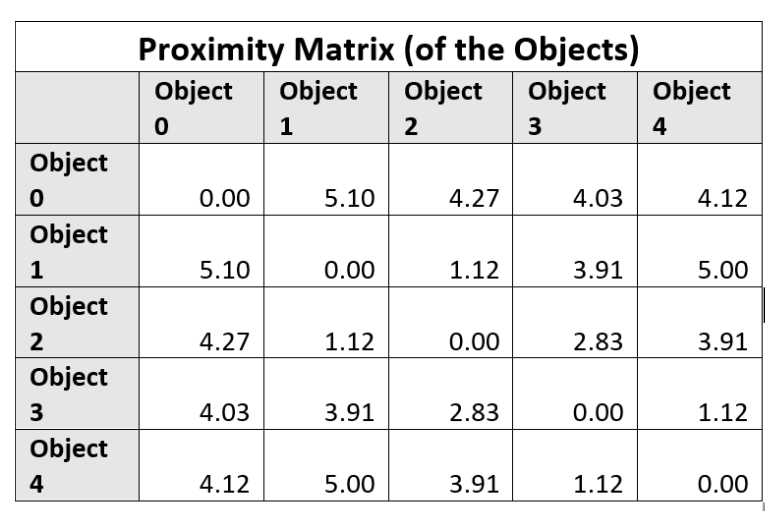
\includegraphics[scale=0.25]{PM.png}
        \caption{Proximity Matrix}
        \label{}
    \end{figure}\end{center}
    \item \textbf{Repeat:}
    \subitem Merge the clusters in the current proximity matrix of the clusters that have the smallest proximity.
    \subitem Update the proximity matrix to reflect the proximity between the new merged cluster and the remaining clusters.
    \item \textbf{Until} only one cluster remains.
\end{enumerate}

\subsection{with Single Linkage}

In \textbf{single linkage algorithms}, the \textbf{proximity between two clusters} is defined as the proximity between the two \underline{closest} points in the two clusters.

\subsubsection*{Downsides of using hierarchical agglomerative clustering with single linkage proximity measure}
\begin{enumerate}
    \item Not as effective in identifying the "main clusters" in datasets where the clusters are not well separated.
    \item Sensitive to outliers and noise. It will in these cases sometimes detect the presence of outliers and noise at the expense of detecting the actual clustering structure.
    \item Algorithm is more computationally complex than k-means.
\end{enumerate}

\subsubsection*{Benefits of using hierarchical agglomerative clustering with single linkage proximity measure}
\begin{enumerate}
    \item You can use it as another means to detect outliers and noise in your dataset.
    \item It can detect:
    \subitem non-convex clusters
    \subitem Clusters of different sparsities
    \subitem Clusters with different number of objects in them
\end{enumerate}

\subsection{with Complete Linkage}
In \textbf{complete linkage algorithms}, the \textbf{proximity between two clusters} is defined as the proximity between the two \underline{furthest away} points in the two clusters.
\subsubsection*{Downsides of using hierarchical agglomerative clustering with complete linkage proximity measure}
\begin{enumerate}[1.]
    \item Tends to split larger clusters, never enabling the algorithm to completely separate the main clusters that we're looking for.
    \item Tends to favor spherical clusters
    \item It tends not to detect noise or outliers.
    \item Has a higher computational complexity than k-means.
\end{enumerate}
\subsubsection*{Benefits of using hierarchical agglomerative clustering with complete linkage proximity measure}
\begin{enumerate}[1.]
    \item It is more robust to noise and outliers.
    \item It does work better for clusters that are not well separated.
\end{enumerate}

\subsection{with Average Linkage}
In \textbf{average linkage algorithms}, the \textbf{proximity between two clusters} is defined as \underline{the average distance} between all pairs of points in the two clusters.

\subsubsection*{Why use average linkage agglomerative hierarchical clustering?}
\begin{enumerate}[1.]
    \item Average linkage strikes a "middle ground" solution in between the results of complete linkage and single linkage.
    \item Less sensitive to noise and outliers than single linkage (but more so than complete linkage).
    \item Less effective at identifying non-convex clusters (or those that are of different sparsities and sizes) than single linkage, but more effective than complete linkage.
    \item Less effective at identifying non well separated clusters than complete linkage (but more effective than single linkage).
    \item Less prone to split large clusters than complete linkage, but more prone than single linkage.
\end{enumerate}

\subsection{with Ward's Linkage}
In \textbf{Ward's linkage algorithms}, the \textbf{proximity between two clusters} is defined as the change in  \underline{objective function} we get when merging the two clusters.\\
(Most common objective function value to use for Ward's linkage is \textbf{inertia}. The initial inertia value of the clustering with all singleton clusters is $0$)

\subsubsection*{Benefits of using Ward's linkage in agglomerative hierarchical clustering.}
\begin{enumerate}[1.]
    \item Tends to identify spherical clusters really well
\end{enumerate}
\subsubsection*{Drawbacks of using Ward's linkage in agglomerative hierarchical clustering.}
\begin{enumerate}[1.]
    \item Tends to favor the same types of clusters that k-means tends to favor (because they both use inertia to define what a cluster is).
    \subitem Spherical clusters.
    \subitem Well separated clusters.
    \subitem Clusters with equal sparsities and the same size.
    \subitem Know the number of clusters that you want
    \subitem Numerical attributes
    \item Also sensitive to noise and outliers
\end{enumerate}







\section{Divisive Hierarchical Clustering}
\subsection{General Algorithm for Divisive Hierarchical Clustering}
\begin{enumerate}[1.]
    \item Split the dataset into 2 or more clusters.
    \item \textbf{Repeat:}
    Select two or more clusters in the current clustering and split each of them into two or more clusters.
    \item \textbf{Until} all objects are in singleton clusters (i.e. clusters of size one).
\end{enumerate}

\subsection{with the Bisecting $k$-Means Algorithm}
\textbf{\underline{Input:}}
\begin{enumerate}[$\bullet$]
    \item Dataset of $m$ objects $X=\{\vec{x}_1,\vec{x}_2,...,\vec{x}_m\}$, where each object $\vec{x}_i=(x_{i1},x_{i2},...,x_{in})$ has $n$ numerical attributes.
    \item Final Number of Desired Clusters in Final Clustering: $K$ [if you don't want the algorithm to end with all
    objects in singleton clusters]
\end{enumerate}
\textbf{\underline{Algorithm:}}
\begin{enumerate}[1.]
    \item \textbf{Initialize} the list of clusters to contain \textbf{the cluster consisting of all points}.
    \item \textbf{Repeat:}
    \subitem[a.] \textbf{Remove a cluster} from the list of clusters\\ (Algorithm specification: how do we select the cluster?)
    \subitem[b.] for $i = 1$ to \underline{\textit{number of trials}} do: Bisect the selected cluster using k-means algorithm (asking for k=2 clusters).
    \subitem[c.] Select the clustering from 2b with \textbf{the lowest inertia}.
    \subitem[d.] Add the two clusters from the clustering selected in 2c to the list of clusters.
    \item Until the list of clusters contains the $K$ that we want.
\end{enumerate}
\textbf{Common ways to choose which cluster to split.}
\begin{enumerate}[1.]
    \item Choose the cluster with the most amount of points in it. (Benefit: you'll end up with more balanced clusters)
    \item Choose the clusters with the highest inertia. (Benefit: you'll end up with a clustering with lower inertia)
\end{enumerate}

\subsubsection*{Why use Bisecting k-means over k-means?}
\begin{enumerate}[-]
    \item Bisecting k-means FORCES there to be a nested clustering structure of your returned clusterings. Just using k-means multiple times (asking for $k=2,3,4, \ldots$ clusters) does not force a nested cluster relationship.
    \item If $k$ is large, then bisecting k-means can find the clustering with $k$ clusters faster than k-means by itself.
\end{enumerate}
\subsubsection*{Cons of Bisecting k-means}
\begin{enumerate}[-]
    \item Bisecting k-means tends to be more computationally complex (than k-means) when the desired cluster number $\mathrm{k}$ is small.
\end{enumerate}


\chapter{Categorical Data Clustering}
\section{Dataset Clustering with Categorical Variables}
\subsection{ t-SNE Algorithm - Using a Distance Matrix Input}
\begin{enumerate}[$\bullet$]
    \item \textbf{\underline{Input:}} $W=[w_{ij}]$ is a $m\times m$ distance matrix that measures the \underline{distance} between each pair of objects in $X=\{\vec{x}_1,...,\vec{x}_m\}$, where the objects in $X$ can be numerical, categorical, or mixed-data type.
    \item \textbf{\underline{Output:}} The projected coordinates $Y=\{\vec{y}_1,...,\vec{y}_m\}$, where each projected coordinate $\vec{y}_i=(y_{i1},y_{i2})$ has 2 attributes where each attribute is numerical.
    \item \textbf{\underline{Basic Idea:}}
    \begin{enumerate}[(1).]
        \item \textbf{Creates an Actual Similarity Matrix $P$ for the Points in the \textit{Original Dataset}.} Similarity between a given point and another point is a function that uses: 1. the normal distribution; 2. the supplied distance metric $w_{ij}$ distance between the two original dataset points.
        \item \textbf{Creates a Similarity Matrix Function of Variables $Q$ for the Points in the \textit{Projected Dataset}.} Similarity between a given point and another point is a function of: 1. the $t$-distribution; 2. the euclidean distance between the two projected dataset points.
        \item \textbf{Find values for $Y=\{\vec{y}_1,...,\vec{y}_m\}$ that minimize $\textnormal{dist}(P,Q)$.}
    \end{enumerate}
\end{enumerate}

\subsection{Creating a Distance Matrix for Datasets with Categorical Variables}
\begin{definition}[Hamming Distance]
    \normalfont
    To measure the distance between objects $\boldsymbol{x}_{\boldsymbol{i}}=\left(x_{i 1}, x_{i 2}, \ldots, x_{i n}\right)$ and $\boldsymbol{x}_{\boldsymbol{i}^{\prime}}=\left(x_{i^{\prime} 1}, x_{i^{\prime} 2}, \ldots, x_{i^{\prime} n}\right)$ where each of the $n$ attributes for a given object are categorical, we can use the Hamming distance.
    $$
    \operatorname{dist}\left(\boldsymbol{x}_{\boldsymbol{i}}, \boldsymbol{x}_{\boldsymbol{i}^{\prime}}\right)=\sum_{j=1}^n \delta\left(x_{i j}, x_{i^{\prime} j}\right)
    $$
    where
    $$
    \delta\left(x_{i j}, x_{i^{\prime} j}\right)=\left\{\begin{array}{ll}
    0, & \text { if } x_{i j}=x_{i^{\prime} j} \\
    1, & \text { if } x_{i j} \neq x_{i^{\prime} j}
    \end{array}\right.
    $$
    In other words, the hamming distance between two objects represents the number of disagreements between two objects of categorical attributes.
\end{definition}
Hamming distance matrix $\mathbf{W}=[w_{ii'}]=[\sum_{j=1}^n \delta\left(x_{i j}, x_{i^{\prime} j}\right)]$

\begin{definition}[Gower's Distance]
    \normalfont
    To measure the distance between objects $\boldsymbol{x}_i=\left(x_{i 1}, x_{i 2}, \ldots, x_{i n}\right)$ and $\boldsymbol{x}_{i^{\prime}}=\left(x_{i^{\prime} 1^{\prime}}, x_{i^{\prime} 2}, \ldots, x_{i^{\prime} n}\right)$ where at least one of the attributes is numerical and at least one is categorical, we can use Gower's distance.
    $$
    \operatorname{dist}\left(\boldsymbol{x}_{\boldsymbol{i}}, \boldsymbol{x}_{\boldsymbol{i}^{\prime}}\right)=\frac{\sum_{j=1}^n \delta\left(x_{i j}, x_{i^{\prime} j}\right)}{n}
    $$
    - If attribute $j$ is categorical, then:
    $$
    \delta\left(x_{i j}, x_{i^{\prime} j}\right)=\left\{\begin{array}{ll}
    0, & \text { if } x_{i j}=x_{i^{\prime} j} \\
    1, & \text { if } x_{i j} \neq x_{i^{\prime} j}
    \end{array}\right.
    $$
    - If attribute $j$ is numerical, then:
    $$
    \delta\left(x_{i j}, x_{i^{\prime} j}\right)=\frac{\left|x_{i j}-x_{i^{\prime} j}\right|}{\max \left(\boldsymbol{x}_{* j}\right)-\min \left(\boldsymbol{x}_{* j}\right)}
    $$
\end{definition}
Gower's distance matrix $\mathbf{W}=[w_{ii'}]=[\frac{\sum_{j=1}^n \delta\left(x_{i j}, x_{i^{\prime} j}\right)}{n}]$

\textbf{Interpretation:} Gower's distance between two objects $\boldsymbol{x}_{\boldsymbol{i}}, \boldsymbol{x}_{\boldsymbol{i'}}$, will be
\begin{enumerate}
    \item $0$ if $\boldsymbol{x}_{\boldsymbol{i}}= \boldsymbol{x}_{\boldsymbol{i'}}$
    \item $1$ if none of the categorical attributes agree and the numerical attributes are the furthest away values in the dataset.
\end{enumerate}

\section{Partitional Clustering Algorithms for Datasets with Categorical Variables}

\subsection{Just Categorical Variables: $k$-Modes Clustering Algorithm}
When our dataset is comprised of \textbf{just categorical variables}, we can use a \textbf{partitional clustering algorithm} known as \textbf{k-modes} to cluster the dataset.
\begin{center}\begin{figure}[htbp]
    \centering
    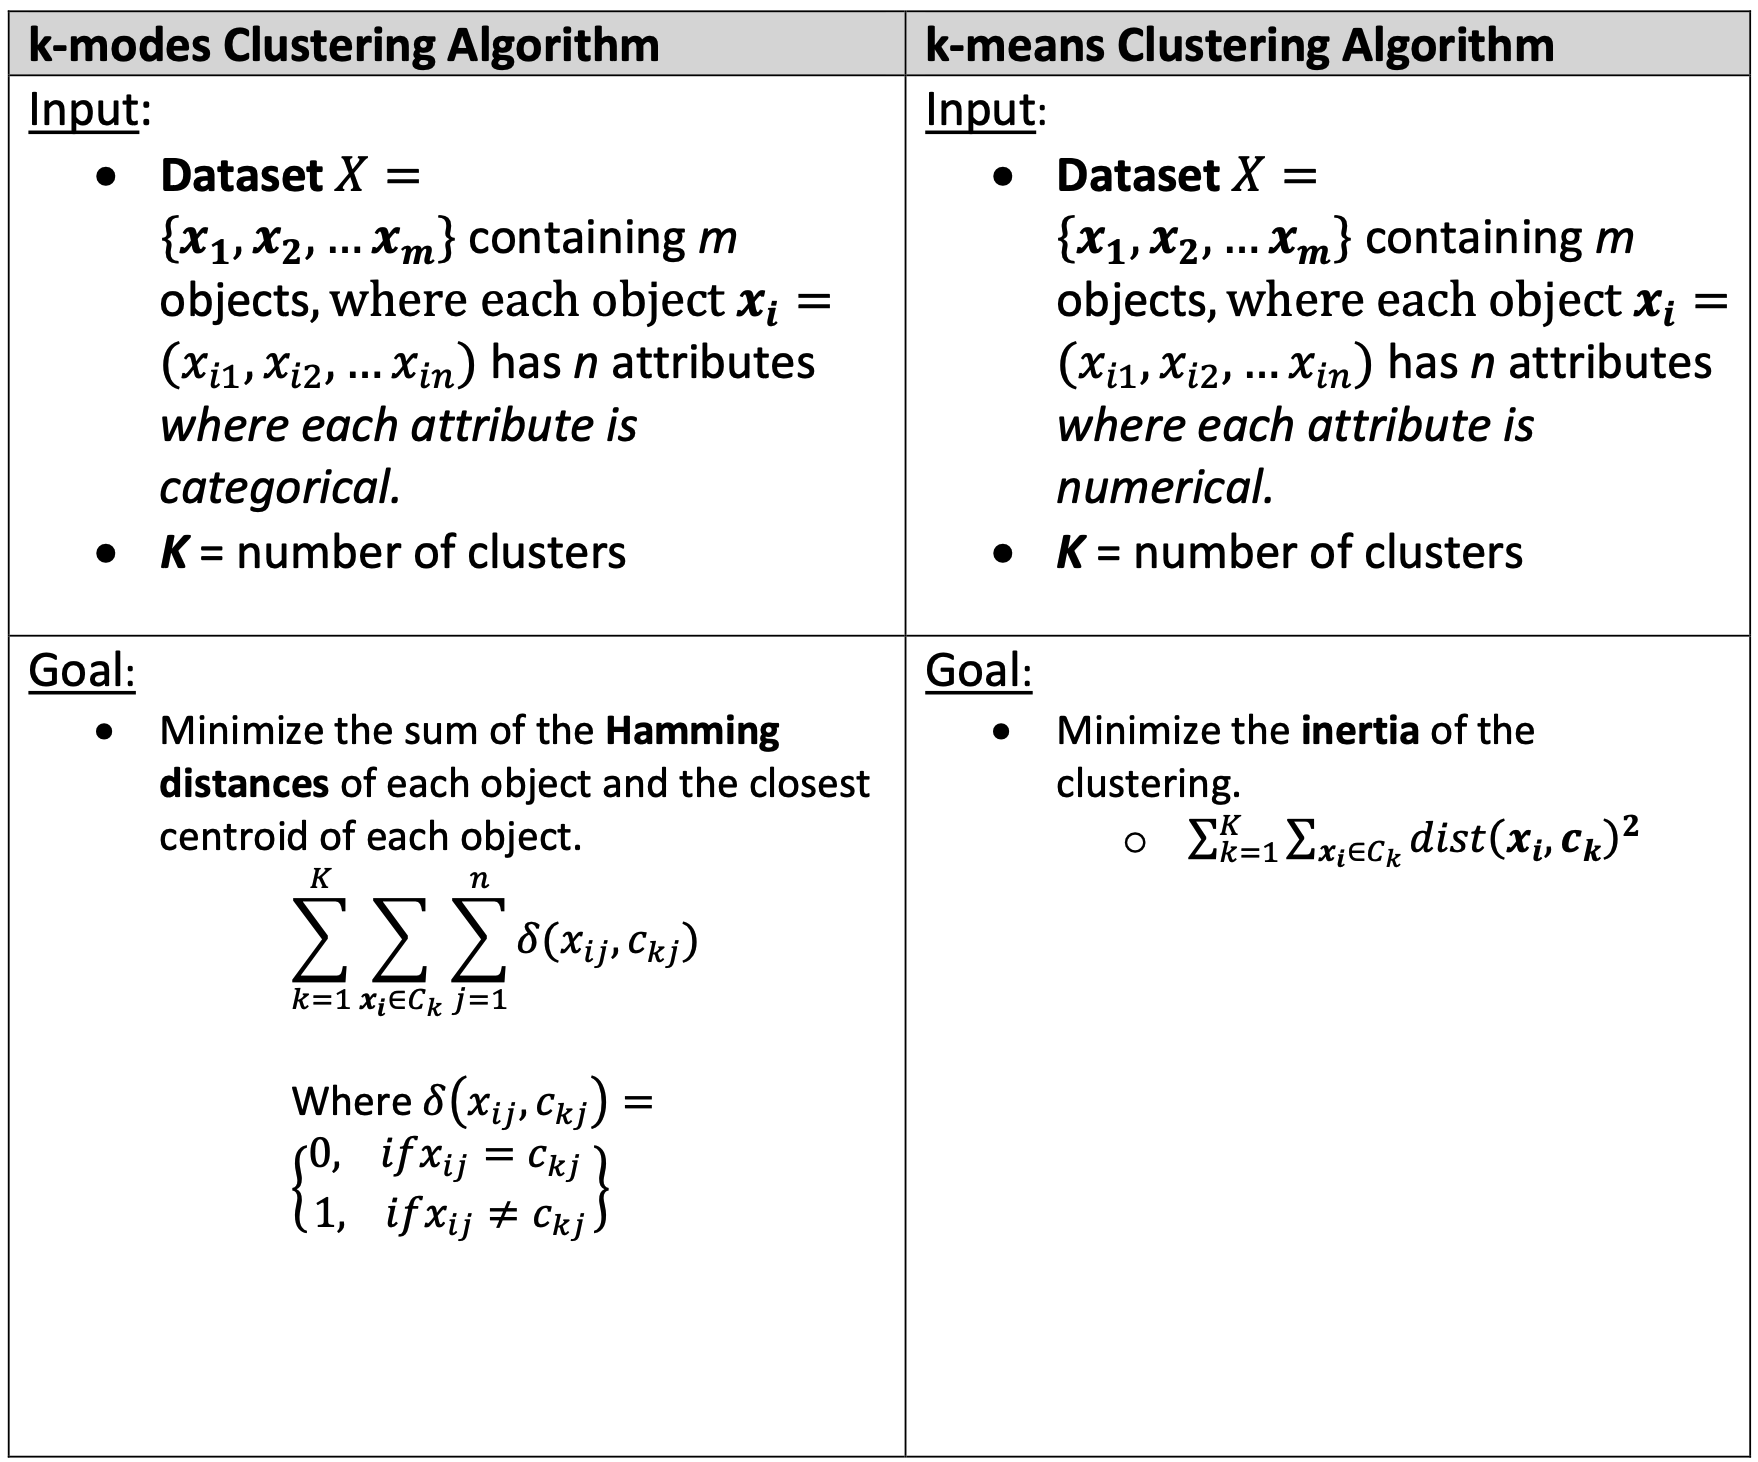
\includegraphics[scale=0.2]{kmodes.png}
    \caption{$k$-modes vs. $k$-means}
    \label{}
\end{figure}\end{center}
We can also use an elbow method for k-modes. Different to k-means, we compute the average Hamming distances instead of inertia (in squared euclidean distance metric).
\subsubsection*{Benefits and Drawbacks of k-modes}
\begin{enumerate}[$\bullet$]
    \item \textbf{Benefits:} 1. Computationally efficient algorithm. 2. Scale well to datasets with Large numbers of objects and attributes.
    \item \textbf{Drawbacks:} 1. K-modes is only designed to work well for pure categorical dataset; 2. Hamming distance metric it is not the most nuanced metric.
\end{enumerate}



\subsection{Numerical and Categorical Variables: $k$-Prototypes Clustering Algorithm}
When our dataset is comprised of \textbf{categorical AND numerical variables}, we can use a \textbf{partitional clustering algorithm} known as \textbf{k-prototypes} to cluster the dataset.
\begin{center}\begin{figure}[htbp]
    \centering
    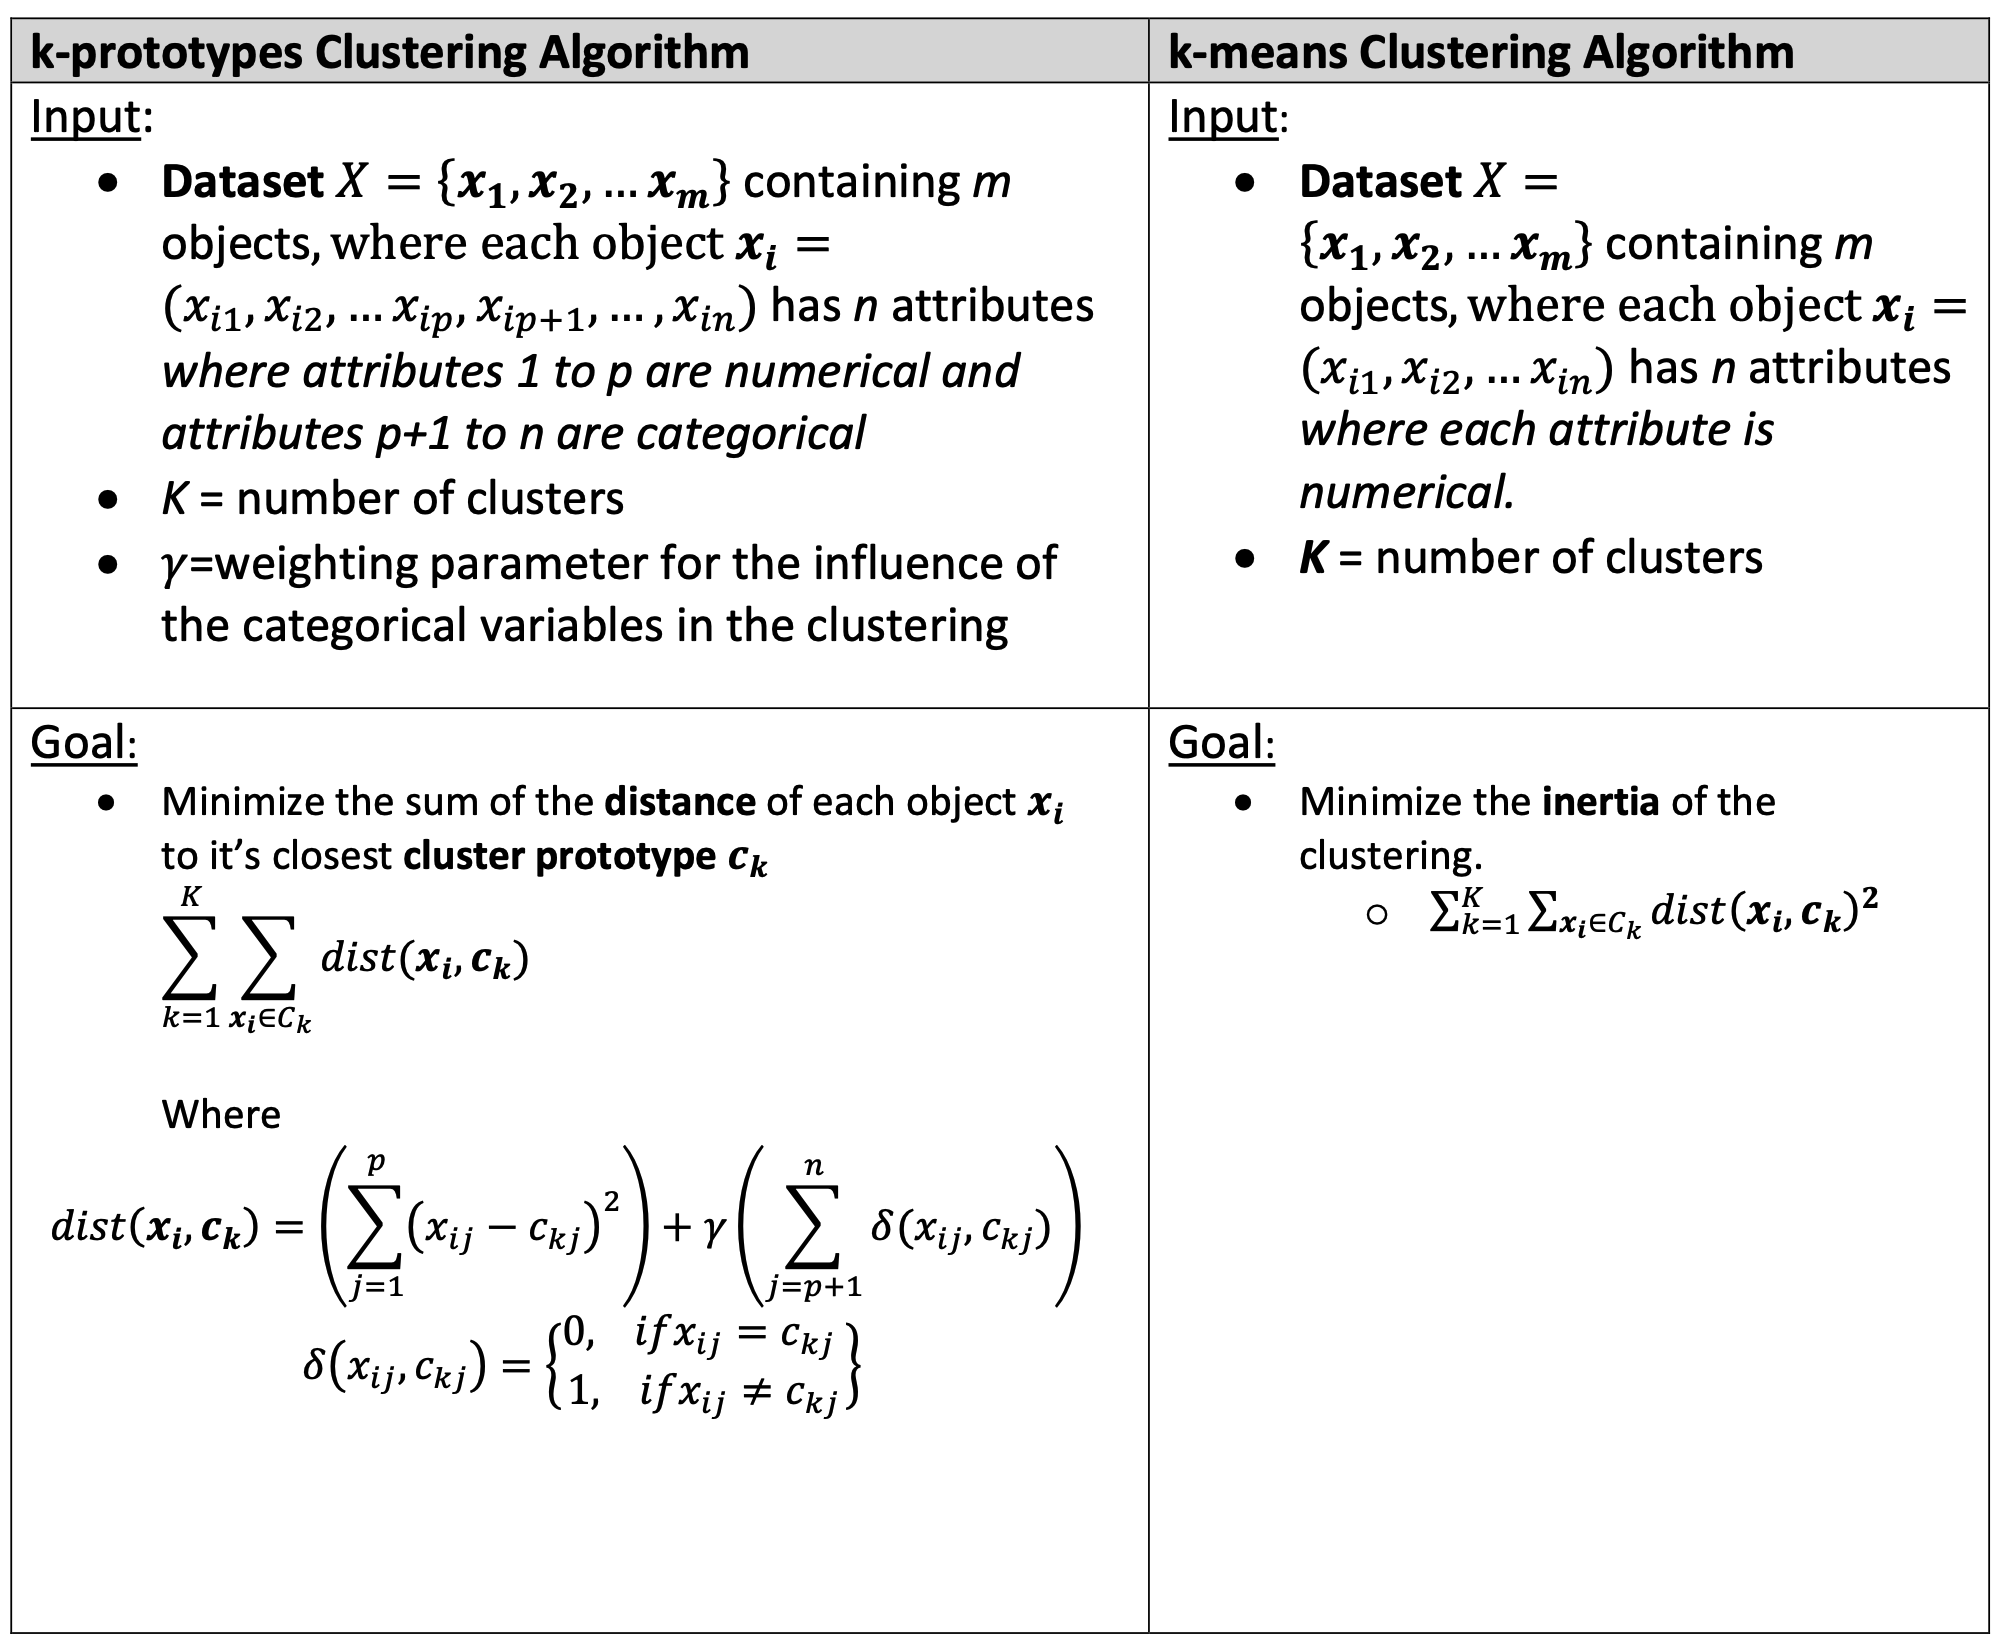
\includegraphics[scale=0.2]{kprototype.png}
    \caption{$k$-prototypes vs. $k$-means}
    \label{}
\end{figure}\end{center}


\section{Hierarchical Clustering Algorithms for Datasets with Categorical Variables}
We only need to change the distance metric by distance matrix for categorical data that showed above.


\chapter{Principal Component Analysis (PCA)}
\begin{enumerate}[$\bullet$]
    \item \underline{Dataset} of $m$ objects $X=\{\vec{x}_1,\vec{x}_2,...,\vec{x}_m\}$, where each object $\vec{x}_i=(x_{i1},x_{i2},...,x_{in})$ has $n$ attributes. We can also think of $X$ as being an $m\times n$ matrix $X_{m\times n}$.
    \item Assume $X_{m\times n}$ has been preprocessed such that the mean of each of the $n$ attributes has been subtracted.
\end{enumerate}
\section{Assumption}
\begin{enumerate}
    \item Variables must be \underline{numerical}.
    \item The relationship between the variables is \underline{linear}.
    \item In order for PCA to produce a reliable result, large enough sample sizes are required. (Rule of thumb: At least 150 samples and 5-10 cases per attribute.)
    \item No significant \underline{outliers}.
\end{enumerate}


\section{Principal component analysis- general goals}
\textbf{Goal: Find some matrix $U_{n\times p}$ such that}
\begin{enumerate}
    \item We can project our $X_{m\times n}$ onto a new matrix $Y_{m\times p}=X_{m\times n}U_{n\times p}$ with $p\leq n$ attributes. Each column of $Y_{m\times p}$ (i.e., the \textbf{projected} attributes $Y_{*j}$) is known as a \textbf{principal component}.
    \item Each pair of \textbf{principal components} (i.e. projected attributes) in $Y_{m\times p}$ has $0$ covariance. $$\textnormal{Cov}(Y_{*j},Y_{*j'})=0 \textnormal{ for }1\leq j\neq j'\leq p$$
    \item The sum of the principal component (i.e. projected attribute) variances of $Y_{m\times p}$ are
    less than or equal to (only equal when $p=n$) the sum of the attribute variances of the original data matrix $X_{m\times n}$, i.e.,
    \begin{equation}
        \begin{aligned}
            \sum_{i=1}^n \textnormal{Var}(X_{*j})\geq \sum_{i=1}^p \textnormal{Var}(Y_{*j})
        \end{aligned}
        \nonumber
    \end{equation}
    \item The first principal component, $Y_{*1}$, captures as much of the total attribute variance (of the original dataset) as possible; The second principal component, $Y_{*2}$, (which is orthogonal to $Y_{*1}$), captures as much of the remaining total variance as possible; The third principal component, $Y_{*3}$, (which is orthogonal to $Y_{*1}$ and $Y_{*2}$), captures as much of the remaining total variance as possible; This process keeps going until, we have $p\leq n$ orthogonal principal components.
\end{enumerate}

\section{Process of PCA}
\begin{enumerate}
    \item Calculate the \textbf{covariance matrix} $C_{n \times n}$ of $X_{m \times n}$.
    \item Calculate the $n$ \textbf{eigenvalues and eigenvectors of covariance matrix $C_{n \times n}$}.
    \item Order the eigenvalues from highest to lowest: $\lambda_1, \lambda_2, \ldots \lambda_n$, then select the $p$ highest eigenvalues (keeping this order).
    \item Order the corresponding $p$ eigenvectors (which will be column vectors of length $n$) that correspond to these $p$ selected eigenvalues in the same order: $\boldsymbol{v}_{* 1}, \boldsymbol{v}_{* 2}, \ldots \boldsymbol{v}_{* p}$
    \item Let $U_{n \times p}=\left[\boldsymbol{v}_{* 1}\left|\boldsymbol{v}_{* 2}\right| \ldots \mid \boldsymbol{v}_{* p}\right]$ we call these eigenvectors the loading vectors.
\end{enumerate}

\section{How Do We Choose $p<n$?}
\begin{center}\begin{figure}[htbp]
    \centering
    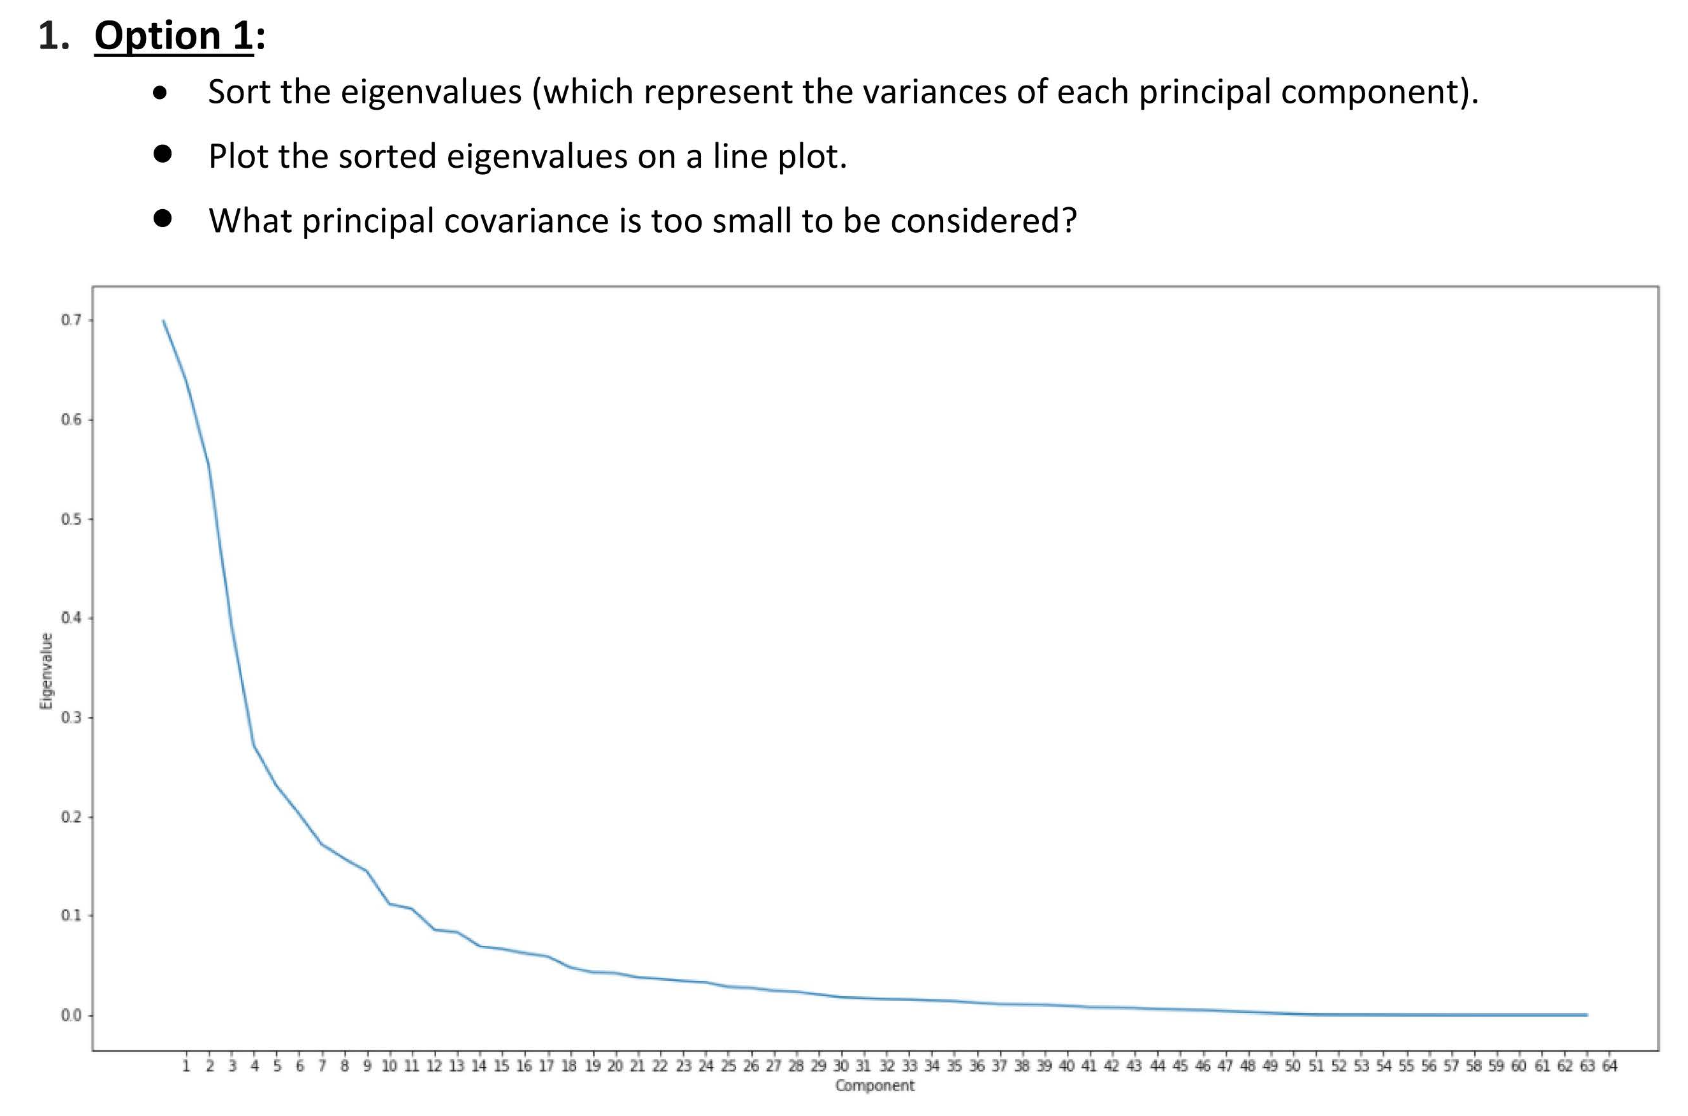
\includegraphics[scale=0.18]{ChooseP.png}
    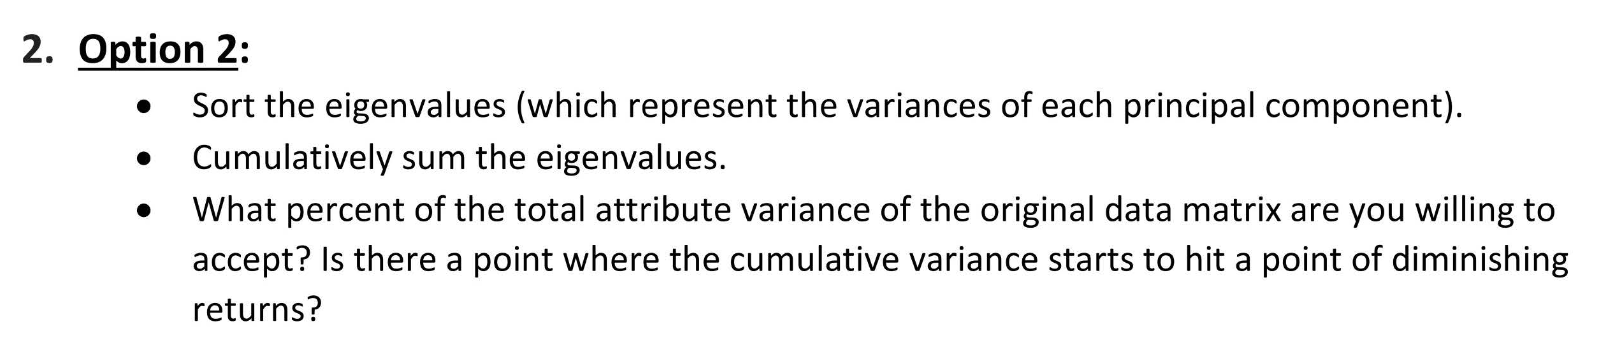
\includegraphics[scale=0.18]{ChooseP2.png}
    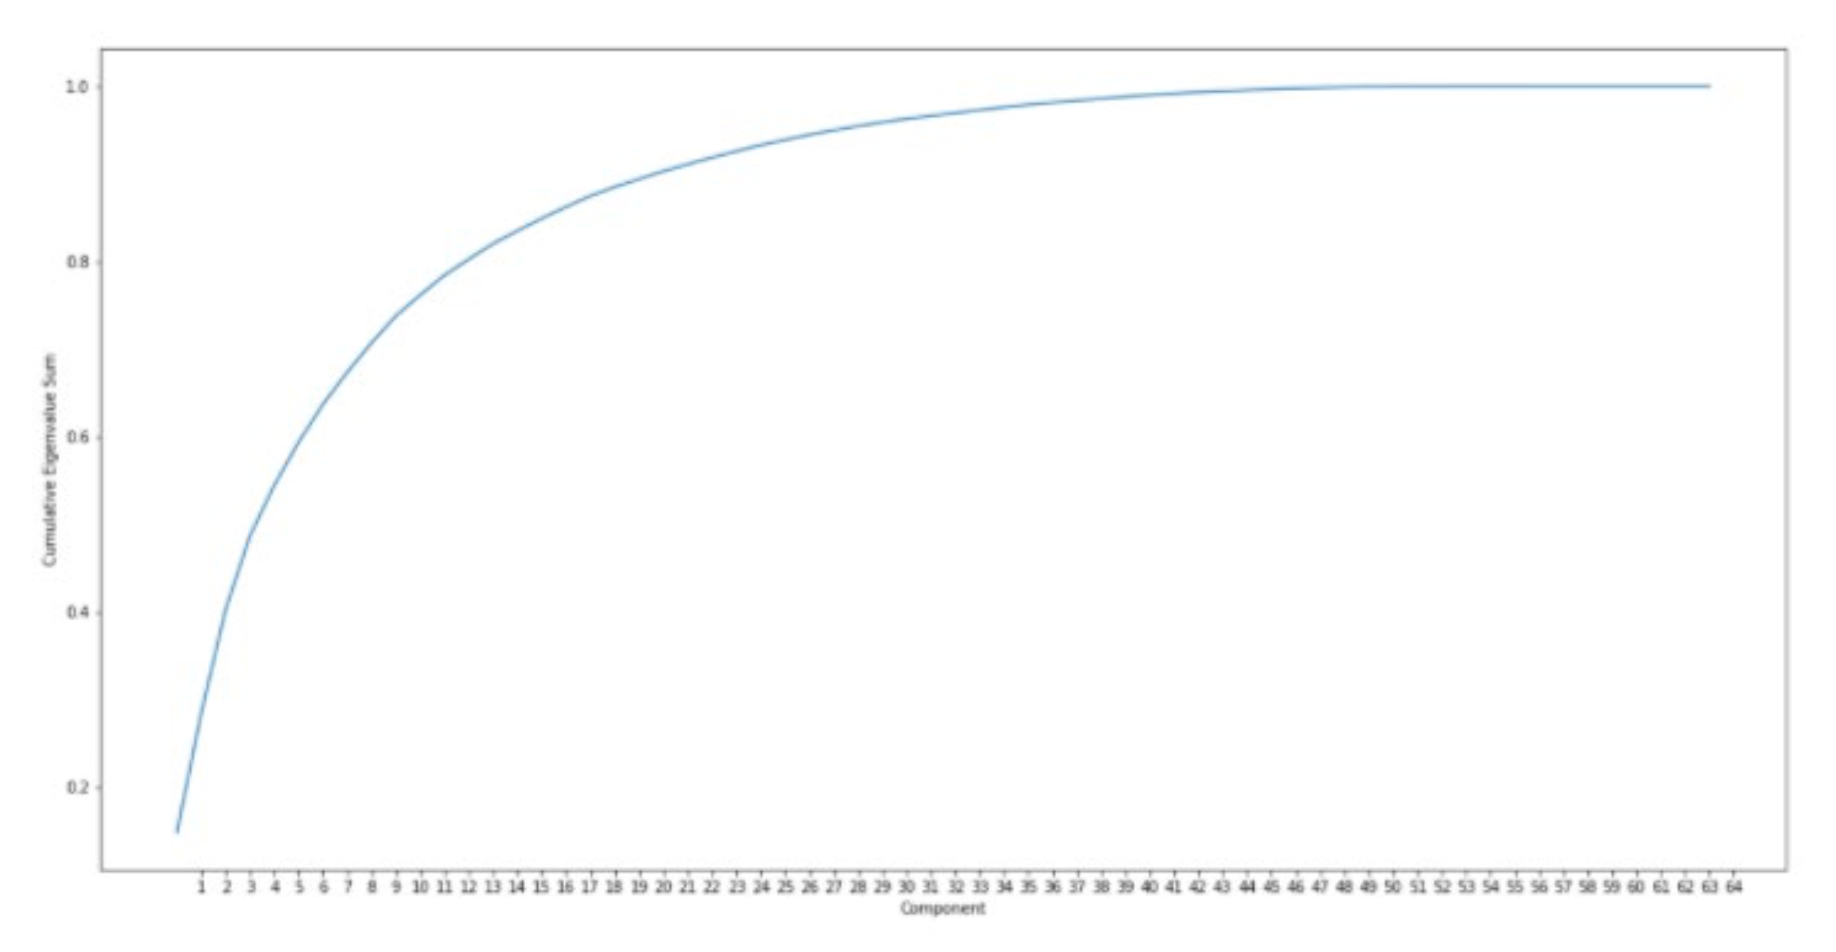
\includegraphics[scale=0.15]{ChooseP3.png}
    \caption{How Do We Choose $p<n$}
    \label{}
\end{figure}\end{center}

\chapter{Gaussian Mixture Models}
\section{Why use model-based clustering?}
Model-based clustering can give us a statistically rigorous model for \textbf{generating new random variable values} from \textbf{the underlying distribution that generated the training dataset that we have}.

\textbf{Goal of Gaussian Mixture Models}
\begin{enumerate}[$\bullet$]
    \item Use maximum likelihood estimation to more rigorously estimate the priors, means, and covariance matrices of each of the $K$ clusters (i.e. Gaussian distributions).
    \item Use these estimations to calculate the probability that each point in the dataset came from each of the respective $K$ clusters (i.e., Gaussian distributions).
\end{enumerate}
We now have a statistically rigorous model for estimating the probability that an object $\vec{x}$ is drawn from each of the $K$ cluster distributions.

\section{Overview of Mixture Models}
\subsection{Assumption of Mixture Model Fitting Given a Dataset}
Data points $X=\{\vec{x}_1,\vec{x}_2,...,\vec{x}_m\}$ have been generated from a random process involving a mixture of $K$ probability distributions. We can think of each of probability distribution $k$ as distributions that generated the data in cluster $C_k$.

\textbf{Assumed Random Process for How the Given Data $X=\{\vec{x}_1,\vec{x}_2,...,\vec{x}_m\}$ was Generated by this way:}

For $i$ in $1$ to $m$:
\begin{enumerate}[1.]
    \item Randomly select one of the $K$ distributions.
    \item Generate an object $\vec{x}_i$ from this distribution.
\end{enumerate}

\textbf{Unknown (Usually) and Goal to Estimate:}
















\section{Gaussian Mixture Models}









\section{Benefits/Drawbacks of Gaussian Mixture Model Clustering (with EM Algorithm)}














\section{How to choose the number of clusters in a Gaussian Mixture Model}







\end{document}